\chapter{Homotopy Groups of the space of Immersions} \label{CH:H}



%%%%%%%%%%%%%% INTRO %%%%%%%%%%%%%%%%%%
This chapter studies the space of immersions of orientable surfaces into parallelizable manifolds.
Specifically, we identify the set of path-components, as well as all homotopy groups, of this space in terms of the homotopy-type of the target manifold and Stiefel spaces. 


We immediately state our main result: 
\begin{mythm}{W} \label{mainhomthm}
For $W_{g}$ a smooth, compact, orientable surface of genus $g$ and $M^{n}$ a smooth, parallelizable manifold of dimension $n > 2$, 
there is an isomorphism between homotopy groups: for $k \geq 1$
\[
\pi_{k}{\sf Imm}(W_{g}, M) \cong 
\pi_{k}M \times (\pi_{k + 1}M)^{2g} \times \pi_{k + 2}M \times 
\pi_{k}\sV_{2}(n) \times (\pi_{k + 1}\sV_{2}(n))^{2g} \times \pi_{k + 2}\sV_{2}(n)~.
\]
For $k = 0,$ there is an action of $\pi_1(M)$ on $\Bigl((\pi_{1}M)_{\rm Com}^{2g} \times \pi_{2}M \Bigr)$
for which there is a bijection:
\[
\pi_{0}{\sf Imm}(W_{g}, M) \cong 
\pi_{0}M \times \Bigl((\pi_{1}M)_{\rm Com}^{2g} \times \pi_{2}M \Bigr)_{/\pi_1(M)}
\times 
\pi_{0}\sV_{2}(n) \times (\pi_{1}\sV_{2}(n))^{2g} \times \pi_{2}\sV_{2}(n)~.
\]
\end{mythm}

\begin{remark}
Here $(\pi_{1}M)_{\rm Com}^{2g}$  is defined to be the set
\[
(\pi_{1}M)^{2g}_{\rm Com} :=
\]
\[ \Big\{ \left([\alpha_{1}], [\beta_{1}], \hdots [\alpha_{g}], [\beta_{g}]\right) \in (\pi_{1}M)^{2g} : [\alpha_{1}, \beta_{1}][\alpha_{2}, \beta_{2}]\hdots[\alpha_{g}, \beta_{g}] = [e] \Big\} \subset (\pi_{1}M)^{2g}
\]
and the action of $\pi_{1}M$ restricted to $(\pi_{1}M)_{\rm Com}^{2g}$ is simultaneous conjugation on each component. The action of $\pi_{1}M$ restricted to $\pi_{2}M$ is the canonical action. However, generally the action of $\pi_{1}M$ on $(\pi_{1}M)_{\rm Com}^{2g} \times \pi_{2}M$ will not be the product of these two simple actions.
\end{remark}

Note the lack of symmetry in regard to $\pi_{0}{\sf Imm}(W_{g}, M),$ namely we might expect 
\[
\pi_{0}{\sf Imm}(W_{g}, M) \cong 
\]
\[
\pi_{0}M \times \Bigl((\pi_{1}M)_{\rm Com}^{2g} \times \pi_{2}M \Bigr)_{/\pi_1(M)}
\times 
\pi_{0}\sV_{2}(n) \times \Bigl( (\pi_{1}\sV_{2}(n))_{\rm Com}^{2g} \times \pi_{2}\sV_{2}(n) \Bigr)_{/\pi_1(\sV_{2}(n))}~.
\]
This is true and agrees with Theorem \ref{mainhomthm}, it is just that $\sV_{2}(n)$ is a \textit{simple} space and therefore $\pi_{1}\sV_{2}(n)$ is abelian which implies $(\pi_{1}\sV_{2}(n))_{\rm Com}^{2g} \cong (\pi_{1}\sV_{2}(n))^{2g}$ and the action of $\pi_{1}\sV_{2}(n)$ on $\Bigl( (\pi_{1}\sV_{2}(n))_{\rm Com}^{2g} \times \pi_{2}\sV_{2}(n) \Bigr)$ is trivial. In the case that $M$ is simple, there is the following reduction in the identification of connected components of ${\sf Imm}(W_{g}, M)$:
\begin{cor} \label{sconcomp}
For $M$ a simple, smooth, parallelizable manifold there is the following bijection:
\[
\pi_{0}{\sf Imm}(W_{g}, M) \cong \pi_{0}M \times (\pi_{1}M)^{2g} \times \pi_{2}M
\times (\pi_{1}\sV_{2}(n))^{2g} \times \pi_{2}\sV_{2}(n) ~.
\]
\end{cor}

 

Another interesting case of Theorem \ref{mainhomthm} is when our target manifold is $4-$dimensional.
\begin{cor} \label{firstc}
For $M^{4}$ a smooth, connected, parallelizable manifold of dimension $4,$ we have the following isomorphisms for $k \geq 1:$
\[
\pi_{k}{\sf Imm}(W_{g}, M^{4}) \cong 
\]
\[
\pi_{k}M \times (\pi_{k + 1}M)^{2g} \times \pi_{k + 2}M \times 
\pi_{k}S^{2} \times (\pi_{k + 1}S^{2})^{2g} \times \pi_{k + 2}S^{2} \times 
\pi_{k}S^{3} \times (\pi_{k + 1}S^{3})^{2g} \times \pi_{k + 2}S^{3}~,
\]
along with the bijection
\[
\pi_{0}{\sf Imm}(W_{g}, M^{4}) \cong  \Bigl((\pi_{1}M)_{\rm Com}^{2g} \times \pi_{2}M \Bigr)_{/\pi_1(M)} 
\times (\pi_{1}S^{2})^{2g} \times (\pi_{1}S^{3})^{2g} \times \pi_{2}S^{2} \times \pi_{2}S^{3}
\]
\[
\cong \Bigl((\pi_{1}M)_{\rm Com}^{2g} \times \pi_{2}M \Bigr)_{/\pi_1(M)} 
\times \ZZ ~.
\]
\end{cor}
\begin{proof}
The Stiefel space $\sV_{2}(4)$ is homeomorphic to the unit tangent bundle of $S^{3}.$ As $S^{3}$ is parallelizable, we have that $\tau_{S^{3}} \approx \epsilon_{S^{3}}^{3}$, and therefore $\sV_{2}(4) \approx S^{3} \times S^{2}.$ 
\end{proof}
Corollary \ref{firstc} shows that one can compute the homotopy groups of ${\sf Imm}(W_{g}, M^{4})$ to the extent that one can compute the homotopy groups of $M, S^{2},$ and $S^{3}.$ In particular, $\pi_{k}{\sf Imm}(W_{g}, \RR^{4})$ can be classified completely in terms of the homotopy groups of $S^{2}$ and $S^{3},$ which for $k \geq 3$ we have that $\pi_{k}S^{2} \cong \pi_{k}S^{3}.$ It's been shown in \cite{IMW} that $\pi_{k}S^{2} \neq 0$ for all $k \geq 1$  and so for $k \geq 3$ we have that 
\[
\pi_{k}{\sf Imm}(W_{g}, \RR^{4}) \cong (\pi_{k}S^{2})^{2} \times (\pi_{k + 1}S^{2})^{4g} \times (\pi_{k + 2}S^{2})^{2} \neq 0~.
\]
Through Corollary \ref{firstc} we also see that the connected components of ${\sf Imm}(W_{g}, \RR^{4})$ simplify drastically to $\pi_{0}{\sf Imm}(W_{g}, \RR^{4}) \cong \pi_{2}(S^{2}) \cong \ZZ.$
The table below records the first few homotopy groups of the space of immersions of $W_{g}$ into $\RR^{4}.$ 

\begin{table}[h!]
\centering
\begin{tabular}{|| c | m{11em} ||}
\hline
$k$ & $\pi_{k}{\sf Imm}(W_{g}, \RR^{4})$     \\
\hline
0 & $\ZZ$  \\
\hline
1 & $\ZZ^{2g + 2}$  \\
\hline
2 & $\ZZ^{4g + 1} \times (\ZZ/2\ZZ)^{2}$  \\
\hline
3 & $\ZZ^{2} \times (\ZZ/2\ZZ)^{4g + 2}$  \\
\hline
4 & $(\ZZ/2\ZZ)^{4g + 2} \times (\ZZ/12\ZZ)^{2}$ \\
\hline
5 & $(\ZZ/2\ZZ)^{4} \times (\ZZ/12\ZZ)^{4g}$ \\
\hline
6 & $(\ZZ/2\ZZ)^{4g + 2} \times (\ZZ/12\ZZ)^{2}$ \\
\hline
7 & $(\ZZ/2\ZZ)^{4g + 2} \times (\ZZ/3\ZZ)^{2}$ \\
\hline
\end{tabular}
\caption{Homotopy Groups of ${\sf Imm}(W_{g}, \RR^{4})$}
\label{table:1}
\end{table}


Higher dimensional tori give other examples of simple, parallelizable manifolds for which Theorem \ref{mainhomthm} applies. With the identification of $\sV_{2}(4) \approx S^{2} \times S^{3},$ we may compute that $\pi_{0}{\sf Imm}(W_{g}, \TT^{4}) \cong \ZZ^{8g + 1}, \pi_{1}{\sf Imm}(W_{g}, \TT^{4}) \cong \ZZ^{2g + 6},$ and $\pi_{k}{\sf Imm}(W_{g}, \TT^{4}) \cong \pi_{k}{\sf Imm}(W_{g}, \RR^{4})$ for $k \geq 2.$ Because $\sV_{2}(3) \cong {\sf SO}(3) \approx \RR P^{3},$ we may compute $\pi_{k}\sV_{2}(3)$ as $S^{3}$ is the universal cover of $\sV_{2}(3)$. This allows us to compute $\pi_{k}{\sf Imm}(W_{g}, \TT^{3})$ for $k$ as large as we can compute $\pi_{k}S^{3}.$ We record the first few homotopy groups of ${\sf Imm}(W_{g}, \TT^{3})$ below.

\begin{table}[h!]
\centering
\begin{tabular}{|| c | m{11em} ||}
\hline
$k$ & $\pi_{k}{\sf Imm}(W_{g}, \TT^{3})$     \\
\hline
0 & $\ZZ^{6g} \times (\ZZ/2\ZZ)^{2g}$ \\
\hline
1 & $\ZZ^{4} \times (\ZZ/2\ZZ) $  \\
\hline
2 & $\ZZ^{2g} \times (\ZZ/2\ZZ)$  \\
\hline
3 & $\ZZ \times (\ZZ/2\ZZ)^{2g + 1}$  \\
\hline
4 & $(\ZZ/2\ZZ)^{2g + 1} \times (\ZZ/12\ZZ)$ \\
\hline
5 & $(\ZZ/2\ZZ)^{2} \times (\ZZ/12\ZZ)^{2g}$ \\
\hline
\end{tabular}
\caption{Homotopy Groups of ${\sf Imm}(W_{g}, \TT^{3})$}
\label{table:11}
\end{table}

The figures below show two embedded genus two surfaces in a 3-torus, $W_{2} \hookrightarrow \TT^{3},$ which do not lie in the same path component of ${\sf Imm}(W_{2}, \TT^{3}).$ Here we represent $\TT^{3}$ as a solid cube with opposite faces identified.



\begin{figure}[h]
\centering
\begin{minipage}{.5\textwidth}
  \centering
  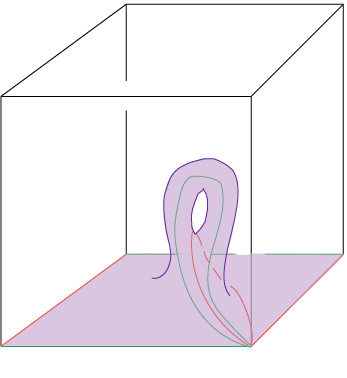
\includegraphics[width=.6\linewidth]{Wg2}
  \captionof{figure}{An embedding $W_{2} \hookrightarrow \TT^{3}$}
  \label{fig:test1}
\end{minipage}%
\begin{minipage}{.5\textwidth}
  \centering
  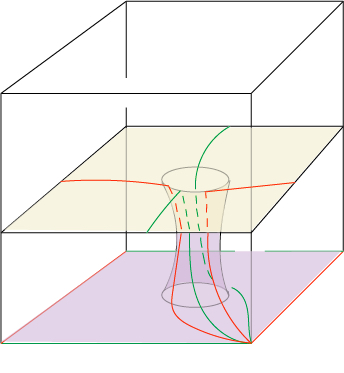
\includegraphics[width=.6\linewidth]{Wg1}
  \captionof{figure}{A different embedding $W_{2} \hookrightarrow \TT^{3}$}
  \label{fig:test2}
\end{minipage}
\end{figure}

The reason that these embeddings lie in different path components is because restricting each embedding to the $1-$skeleton, which are colored red and green in the figures, yield different elements of $(\pi_{1}\TT^{3})^{4}.$



Next, we identify a weak homotopy equivalence between ${\sf Imm}(W_{g}, M)$ and mapping spaces which will have computable homotopy groups.


%%%%%%%%%%%% STRUCTURE OF ARGUMENT %%%%%%%%%%%%%%%
\section{A Homotopy Equivalence Between Bundle Injections and Mapping Spaces} 
Recall that by the Hirsch-Smale Theorem \ref{hst} we have that ${\sf Imm}(W_{g}, M)$ is weakly homotopy equivalent to ${\sf Imm^{f}}(W_{g}, M),$ the space of \textit{formal immersions} which we defined (Definition \ref{formalimmdef}) as fiberwise bundle injections between tangent bundles: 
\[
{\sf Imm^{f}}(W_{g}, M) := {\sf BunInj}(\tau_{W_{g}}, \tau_{M})~.
\]
Under our assumption that $M$ is parallelizable, we have that there is a homeomorphism 
\begin{equation} \label{eq1new}
{\sf Imm^{f}}(W_{g}, M) := {\sf BunInj}(\tau_{W_{g}}, \tau_{M}) \xra{\approx} {\sf BunInj}(\tau_{W_{g}}, \epsilon_{M}^{n})
\end{equation}
from a choice of trivialization of the tangent bundle of $M.$


\begin{convention} \label{cov1}
Recall from Convention \ref{cccc} that we endow ${\sf Map}(X, Y)$ with the appropriate topology depending on whether or not $X$ and $Y$ are smooth manifolds. Natural subspaces such as immersions, ${\sf Imm}(W_{g}, M) \hookrightarrow {\sf Imm^{f}}(W_{g}, M) \subset {\sf Map}(\sT W_{g}, \sT M),$ or based maps ${\sf Map}_{\ast}(X, Y) \subset {\sf Map}(X, Y),$ will be equipped with the subspace topology. Similarly, we equip both ${\sf BunInj}(\tau_{W_{g}}, \tau_{M}) \subset {\sf Map}(TW_{g}, TM)$ and ${\sf BunInj}_{/W}(E \rightarrow W, E' \rightarrow W) \subset {\sf Map}(E, E')$ with the appropriate subspace topology.
\end{convention}




\begin{lemma} \label{lem.homeo}
There is a homeomorphism between spaces 
\[
h: {\sf Map^{smooth}}(W_{g}, M) \times {\sf BunInj}_{/W_{g}}(\tau_{W_{g}}, \epsilon_{W_{g}}^{n}) \rightarrow {\sf BunInj}(\tau_{W_{g}}, \epsilon_{M}^{n})
\]
given by 
\[\left( (W_{g} \xra{f} M), \left(\begin{tikzcd}
TW_{g} \arrow[rd] \arrow[r, "F"]  & \RR^{n} \times W_{g} \arrow[d]\\
& W_{g}
\end{tikzcd} \right) \right)
\mapsto \left(
\begin{tikzcd}
TW_{g} \arrow[rd] \arrow[r, "F"] & \RR^{n} \times W_{g} \arrow[d]  \arrow[r, "id \times f"]& \RR^{n} \times M \arrow[d] \\
& W_{g} \arrow[r, "f"] & M
\end{tikzcd} \right)~.
\]
\end{lemma}

\begin{proof}
The map $h$ is continuous as it the composition of continuous maps with regard to the topologies in Convention \ref{cov1}.
We can define the inverse map as follows:
\[
h^{-1}\left(\begin{tikzcd}
TW_{g} \arrow[d] \arrow[r, "F"]  & \RR^{n} \times M \arrow[d]\\
W_{g} \arrow[r, "f"] & M
\end{tikzcd} \right) =
\left( (W_{g} \xra{f} M), \left(\begin{tikzcd}
TW_{g} \arrow[rd] \arrow[r, "\tilde{F}"]  & \RR^{n} \times W_{g} \arrow[d]\\
& W_{g}
\end{tikzcd} \right) \right)
\]
where for $v \in T_{x}W_{g}$ we have that $\tilde{F}(v, x) = (F_{x}(v), x) \in \RR^{n} \times W_{g}.$ 
This is again a continuous map and therefore $h$ is a homeomorphism.
\end{proof}


\begin{definition}
Given continuous maps $A \xra{f} C$ and $B \xra{g} C$ we defined the \bit{homotopy pullback} of these maps to be 
\[
A \times_{C}^{h} B := A \times_{C} C^{I} \times_{C} B = \{(a, \gamma, b): f(a) = \gamma(0), g(b) = \gamma(1) \}
\]
along with the projection maps:
\[
\xymatrix{
A \times_{C}^{h} B \ar[rr]^-{{\sf proj}_{B}} \ar[d]^-{{\sf proj}_{A}}
&&
B \ar[d]^-{g}
\\
A \ar[rr]^-{f}
&&
C~.
}
\]
In the case that $A = \ast$ and $f$ selects out the point $c_{0} \in C$, this homotopy pullback is the \bit{homotopy fiber} of $g$ over $c_{0}$ and we denote it as ${\sf hofib}_{c_{0}}(B \xra{g} C).$ 
\end{definition}

We will use properties of homotopy pullbacks frequently in this dissertation.

\begin{remark} \label{rem.hpull}
Recall that a homotopy commutative diagram
\[
\xymatrix{
D \ar[rr]^-{\varphi_{B}} \ar[d]^-{\varphi_{A}}
&&
B \ar[d]^-{g}
\\
A \ar[rr]^-{f}
&&
C~.
}
\]
is called a homotopy pullback diagram if the associated map $D \xra{\varphi} A \times_{C}^{h} B$ from Proposition \ref{diagram.to.map} is a homotopy equivalence.
This alternative definition of a homotopy pullback will often be much more convenient to work with.
\end{remark}


We will now discuss how one can think of the tangent bundle of $W_{g}$ as an element of ${\sf Map}(W_{g}, {\sf BO}(2)).$ Choose some embedding $e: W_{g} \hookrightarrow \RR^{N}$ so that $e(W_{g}) \subset \RR^{N}$ is a smooth submanifold. Then define the map 
\[
Te: W_{g} \rightarrow {\sf Gr}_{2}(N); \hspace{20pt} p \mapsto \big(T_{e(p)}e(W_{g}) \subset T_{e(p)}\RR^{N} = \RR^{N}\big)~.
\]
Then the map
\[
\tau_{W_{g}}: W_{g} \xra{Te} {\sf Gr}_{2}(N) \hookrightarrow {\sf Gr}_{2}(\infty) = {\sf BO}(2)
\]
describes an element in ${\sf Map}(W_{g}, {\sf BO}(2)).$ By the Whitney Embedding Theorem, this map $\tau_{W_{g}}$ is independent of the choice of embedding up to homotopy.

Therefore, it makes sense to consider the homotopy fiber of the map \[
{\sf Map}(W_{g}, {\sf Gr_{2}}(n)) \xra{\gamma_{2} \circ -} {\sf Map}(W_{g}, {\sf BO}(2))\] over $\tau_{W_{g}}$ where $\gamma_{2}$ is the natural inclusion $\Gr_2(n) \hookrightarrow \Gr_{2}(\infty) = {\sf BO}(2).$ We take this homotopy fiber as the definition of ${\sf Map}_{/{\sf BO}(2)}(W_{g}, \Gr_2(n)),$ i.e.
\[
{\sf Map}_{/{\sf BO}(2)}(W_{g}, \Gr_2(n)) := {\sf hofib}_{\tau_{W_{g}}}({\sf Map}(W_{g}, \Gr_{2}(n)) \xra{\gamma_{2} \circ } {\sf Map}(W_{g}, {\sf BO}(2))).
\]





\begin{observation} \label{obsl0}
Applying Equation (\ref{l0m}) to $W_{g},$ we have the canonical homotopy-equivalence:  
\[
{\sf BunInj}_{/W_{g}}(\tau_{W_{g}}, \epsilon_{W_{g}}^{n}) \rightarrow {\sf Map}_{/{\sf BO}(2)}(W_{g}, \Gr_2(n))~.
\]
Specifying an orientation $\sigma$ on $W_{g},$ Equation (\ref{l1m}) give the canonical homotopy-equivalence:
\[
{\sf BunInj}_{/W_{g}}(\tau_{W_{g}}, \epsilon_{W_{g}}^{n}) \rightarrow {\sf Map}_{/{\sf BSO}(2)}(W_{g}, \Gr_2^{\sf or}(n))~.
\]
\end{observation}


\begin{remark} \label{rrr}
Recall that by the Smooth Approximation Theorem \cite{Woc} there is a homotopy equivalence ${\sf Map^{smooth}}(X, Y) \simeq {\sf Map}(X, Y).$
\end{remark}

To summarize what we have done in this section, we have shown that there is a weak homotopy equivalence 
\begin{equation} \label{heeq}
{\sf Imm}(W_{g}, M) \xra[\simeq]{\text{Theorem }\ref{hst}} {\sf Imm^{f}}(W_{g}, M) \xra[\simeq]{\text{Lemma }\ref{lem.homeo}} {\sf Map^{smooth}}(W_{g}, M) \times {\sf BunInj}_{/W_{g}}(\tau_{W_{g}}, \epsilon_{W_{g}}^{n}) 
\end{equation}
\[
\xra[\simeq]{\text{Remark } \ref{rrr} \times \text{Observation }\ref{obsl0}} {\sf Map}(W_{g}, M) \times {\sf Map}_{/{\sf BSO}(2)}(W_{g}, \Gr_2^{\sf or}(n)).
\]

We will examine the homotopy groups of each of these factors in later sections. Our method of attack will be to first calculate $\pi_{k}{\sf Map}(W_{g}, Z)$ for $Z$ a general based topological space. Then we identify a homotopy equivalence ${\sf Map}_{/{\sf BSO}(2)}(W_{g}, \Gr_2^{\sf or}(n)) \simeq {\sf Map}(W_{g}, \sV_{2}(n)).$









\section{Homotopy Groups of Mapping Spaces}
In this section we relate the homotopy groups of ${\sf Map}(W_{g}, Z)$ to the homotopy groups of $Z,$ where $Z$ is a based, path-connected topological space. We begin with the homotopy groups $\pi_{k}{\sf Map}(W_{g}, Z)$ for $k > 0$, and deal with the set of path components, $\pi_{0}{\sf Map}(W_{g}, Z),$ in the next section.

\begin{lemma} \label{moreuniqlemma1}
For based topological spaces $(X, x_{0}), (Y, y_{0})$ we have that the following spaces are homotopy equivalent:
\[
{\sf Map}(X, \Omega_{y_{0}}Y) \simeq {\sf Map}_{\ast}(X, \Omega_{y_{0}}Y) \times \Omega_{y_{0}}Y
\]
where we take the constant map $S^{1} \rightarrow Y$ at $y_{0}$ to be the base point of $\Omega_{y_{0}}Y.$
\end{lemma}
\begin{proof}
Consider the map 
\[
F \colon {\sf Map}(X, \Omega_{y_{0}}Y) \longrightarrow {\sf Map}_{\ast}(X, \Omega_{y_{0}}Y) \times \Omega_{y_{0}}Y; \hspace{15pt} f \mapsto ((f(x_{0}))^{\ast}f, f(x_{0}))
\]
where $(f(x_{0}))^{\ast} \in \Omega_{y_{0}}Y$ is the loop $f(x_{0})$ with the opposite orientation.
Now consider the map
\[
G \colon {\sf Map}_{\ast}(X, \Omega_{y_{0}}Y) \times \Omega_{y_{0}}Y \longrightarrow {\sf Map}(X, \Omega_{y_{0}}Y); \hspace{15pt} (g, \gamma) \mapsto \gamma g~.
\]
We will show that $F \circ G \simeq \id_{({\sf Map}_{\ast}(X, \Omega_{y_{0}}Y) \times \Omega_{y_{0}}Y)}$ and $G \circ F \simeq \id_{{\sf Map}(X, \Omega_{y_{0}}Y)}.$ First
\[
(F \circ G)(g, \gamma) = ((\gamma g(x_{0}))^{\ast}(\gamma g), \gamma g(x_{0})) = ((\gamma \gamma_{y_{0}})^{\ast}(\gamma g), \gamma \gamma_{y_{0}}) = (\gamma_{y_{0}}^{\ast} \gamma^{\ast} \gamma g, \gamma \gamma_{y_{0}}) \simeq (g, \gamma)
\]
where the last homotopy is due to $\gamma \gamma_{y_{0}} \simeq \gamma$ and $\gamma^{\ast} \gamma \simeq \gamma_{y_{0}}.$ Lastly,
\[
(G \circ F)(f) = f(x_{0})(f(x_{0}))^{\ast}f \simeq f
\]
showing that $F$ and $G$ are homotopy inverses proving our claim.
\end{proof}

\begin{observation} \label{oooo}
Note that the argument above can also be used to show that for a based space $(X, x_{0})$ and a topological group $G,$ that 
\[
{\sf Map}(X, G) \simeq {\sf Map}_{\ast}(X, G) \times G~.
\]
\end{observation}

\begin{lemma} \label{moreuniqlemma2}
For based topological spaces $(X, x_{0}), (Y, y_{0})$ in which $x_{0} \in X$ has a neighborhood that deformation retracts onto $\{x_{0}\},$ we have that for $k \geq 1$ there is an isomorphism of groups: 
\[
\pi_{k}{\sf Map}(X, Y) \cong \pi_{k}{\sf Map}_{\ast}(X, Y) \times \pi_{k}Y~,
\]
where we take the constant map at $y_{0}$ to be the base point of ${\sf Map}_{\ast}(X, Y)$ and ${\sf Map}(X, Y).$
\end{lemma}
\begin{proof}
Consider the following pullback diagram, 
\begin{equation} \label{sumdiag}
\xymatrix{
{\sf Map}_{\ast}(X, Y) \ar[rr]^-{} \ar[d]^-{}
&&
{\sf Map}(X, Y) \ar[d]^-{ev_{x_{0}}}
\\
\ast \ar[rr]^-{\langle y_{0} \rangle} 
&&
Y ~.
}
\end{equation}
The assumption ensures $\ast \xra{x_{0}} X$ is a cofibration. Therefore, $ev_{x_{0}}$ is a fibration and thus (\ref{sumdiag}) is a homotopy pullback.
So from (\ref{sumdiag}) we get the associated long exact sequence on homotopy groups:
\[
\xymatrix{
\hdots \ar[r]^-{}
&
\pi_{k + 1}{\sf Map}_{\ast}(X, Y) \ar[rr]^-{} 
&&
\pi_{k + 1}{\sf Map}(X, Y) \ar[rr]^-{}
&&
\pi_{k + 1}Y \ar[dllll]^{\partial_{k}}
&
\\
&
\pi_{k}{\sf Map}_{\ast}(X, Y) \ar[rr]^-{} 
&&
\pi_{k}{\sf Map}(X, Y) \ar[rr]^-{}
&&
\pi_{k}Y \ar[r]^-{}
&
\hdots 
}
\]
Note that we have a section of spaces
\[
s:Y \rightarrow {\sf Map}(X, Y); \hspace{15 pt} y \mapsto ( {\sf const}_{y}: X \rightarrow Y)~,
\] that is $ev_{x_{0}} \circ s = id_{Y}.$ This induces a section of homotopy groups $s^{\ast}: \pi_{k}Y \rightarrow \pi_{k}{\sf Map}(X, Y)$ and implies that $ev_{x_{0}}^{\ast}$ will be surjective and therefore all boundary maps are trivial, $\partial_{k} = 0.$ 
Therefore our long exact sequence is divided into short exact sequences of the form:
\begin{equation} \label{moruniq}
0 \longrightarrow \pi_{k}{\sf Map}_{\ast}(X, Y) \longrightarrow \pi_{k}{\sf Map}(X, Y) \longrightarrow \pi_{k}Y \longrightarrow 0~.
\end{equation} 
For $k \geq 2,$ the existence of $s^{\ast}$ and the Splitting Lemma immediately implies that (\ref{moruniq}) splits:
\[
\pi_{k}{\sf Map}(X, Y) \cong \pi_{k}{\sf Map}_{\ast}(X, Y) \times \pi_{k}Y ~.
\]
For $k = 1,$ we can rewrite (\ref{moruniq}) as 
\[
0 \longrightarrow \pi_{0}{\sf Map}_{\ast}(X, \Omega_{y_{0}}Y) \longrightarrow \pi_{0}{\sf Map}(X, \Omega_{y_{0}}Y) \longrightarrow \pi_{0}\Omega_{y_{0}}Y \longrightarrow 0
\]
and Lemma \ref{moreuniqlemma1} implies that this short exact sequence is split as a product as well. Therefore for $k \geq 1$ we have that 
\[
\pi_{k}{\sf Map}(X, Y) \cong \pi_{k}{\sf Map}_{\ast}(X, Y) \times \pi_{k}Y~.
\]
\end{proof}


\begin{remark}
Dual to the definition of homotopy pullback, there is the notion of \textbf{homotopy pushout} for which we gave an explicit definition in Chapter \ref{CH:B}. One property we will use frequently is that if the following diagram is a pushout:
\[
\xymatrix{
W \ar[rr]^-{f} \ar[d]^-{g}
&&
X \ar[d]^{j}
\\
Y \ar[rr]^{k}
&&
Z
}
\]
and either $f$ or $g$ are cofibrations, then it also realizes a homotopy pushout diagram.
\end{remark}

\subsection{Geometric Crux}
The following geometric argument is the insight which enabled us to consider homotopy groups of ${\sf Imm}(W_{g}, M)$ for arbitrary $g \geq 0.$ This extends Smale's result \cite{Sm3} which identifies the homotopy groups for genus 0, i.e. $\pi_{k}{\sf Imm}(S^{2}, M).$ We start by recalling the definitions of some basic operations on pointed topological spaces.

\begin{definition}
Let $(Z, z_{0})$ be a pointed topological space. The \textit{reduced suspension} of $Z$ is defined to be 
\[
\Sigma Z := (Z \times I)/ \Big((Z \times \{0\}) \cup (\{z_{0}\} \times I) \cup (Z \times \{1\}) \Big)
\] 
where $I = [0, 1].$
\end{definition}

\begin{definition}
Given pointed topological spaces $(Z, z_{0})$ and $(W, w_{0}),$ the wedge sum of $Z$ and $W$ is defined as 
\[
Z \vee W := (Z \sqcup W)/(\{z_{0}\} \sim \{w_{0}\})~.
\]
We denote the iterated wedge sum of $(Z, z_{0})$ with itself $n-$times as $Z^{\vee n}.$
\end{definition}

\begin{observation} \label{ooooo}
Consider the following pushout diagram,
\begin{equation}\label{classicpushout}
\xymatrix{
\partial \DD^{2} = S^{1} \ar[rr]^-{c} \ar[d]^-{i}
&&
(S^{1})^{\vee 2g} \ar[d]^-{}
\\
\DD^{2} \ar[rr]^-{} 
&&
W_{g}~,
}
\end{equation}
where $[c] \in \pi_{1}((S^{1})^{\vee 2g})$ is the product of commutators $a_{1}b_{1}a_{1}^{-1}b_{1}^{-1} \hdots a_{n}b_{n}a_{n}^{-1}b_{n}^{-1}.$ As the inclusion $i: \partial \DD^{2} \rightarrow \DD^{2}$ is a cofibration, the diagram is a homotopy pushout diagram.
\end{observation}




\begin{lemma} \label{geom.crux}
There is a homotopy equivalence between spaces,
\[
\Sigma W_{g} \simeq \Sigma \big( S^{2} \vee (S^{1})^{\vee 2g}\big)~. 
\]
\end{lemma}
\begin{proof}
Taking the reduced suspension of all spaces and maps in diagram (\ref{classicpushout}) results in the homotopy pushout diagram:
\begin{equation} \label{anothalabel}
\xymatrix{
\Sigma S^{1} \simeq S^{2} \ar[rr]^-{\Sigma c} \ar[d]^-{\Sigma i}
&&
\Sigma (S^{1})^{\vee 2g} \ar[d]^-{}
\\
\Sigma \DD^{2} \ar[rr]^-{} 
&&
\Sigma W_{g}~.
}
\end{equation} 
Note that the homomorphism 
\[
\langle a_{1}, b_{1}, \hdots, a_{n}, b_{n} \rangle = \pi_{1}\big((S^{1})^{\vee 2g}\big) \xra{\Sigma} \pi_{2}\big(\Sigma(S^{1})^{\vee 2g}\big); \hspace{20pt}  [\gamma] \mapsto [\Sigma \gamma]
\]
must factor through the abelianization of $\pi_{1}\big((S^{1})^{\vee 2g}\big)$ since $\pi_{2}\big(\Sigma(S^{1})^{\vee 2g}\big)$ is abelian. That is, there exists a unique map such that the following diagram commutes,
\[
\begin{tikzcd}
\langle a_{1}, b_{1}, \hdots, a_{n}, b_{n} \rangle = \pi_{1}\big((S^{1})^{\vee 2g}\big) \arrow[r, "q"] \arrow[rd, "\Sigma"]
&  \pi_{1}\big((S^{1})^{\vee 2g}\big)_{Ab} \cong \ZZ^{2g} \arrow[d, "!"] \\
&  \pi_{2}\big(\Sigma(S^{1})^{\vee 2g}\big)
\end{tikzcd}
\]
where the map $q$ is the canonical quotient map. Now clearly $[c] = a_{1}b_{1}a_{1}^{-1}b_{1}^{-1} \hdots a_{n}b_{n}a_{n}^{-1}b_{n}^{-1}$ is in the kernel of $q$ and therefore it is also in the kernel of $\Sigma,$ i.e. $\Sigma c$ is homotopic to the constant map at the basepoint.
Now in (\ref{anothalabel}), we have identified 
\[
\Sigma W_{g} = {\sf hopush} \left( \begin{tikzcd}
\Sigma S^{1} \arrow[r, "\Sigma c"] \arrow[d, "\Sigma i"] & \Sigma\big( (S^{1})^{\vee 2g} \big) \\
\Sigma \DD^{2}
\end{tikzcd} \right).
\] As this is a homotopy pushout, we may replace any spaces with homotopy equivalent spaces and any maps with homotopic maps and the resulting homotopy pushout will be homotopy equivalent. 
Therefore 
\[
\Sigma W_{g} = {\sf hopush} \left( \begin{tikzcd}
\Sigma S^{1} \arrow[r, "\Sigma c"] \arrow[d, "\Sigma i"] & \Sigma\big( (S^{1})^{\vee 2g} \big) \\
\Sigma \DD^{2}
\end{tikzcd} \right) \simeq 
{\sf hopush} \left( \begin{tikzcd}
\Sigma S^{1} \arrow[r, "{\sf const}_{\ast}"] \arrow[d, "!"] & \Sigma\big( (S^{1})^{\vee 2g} \big) \\
\ast
\end{tikzcd} \right) \simeq
\] 
\[ 
\Sigma \left( {\sf hopush} \left( \begin{tikzcd}
S^{1} \arrow[r, "{\sf const}_{\ast}"] \arrow[d, "!"] & \big((S^{1})^{\vee 2g} \big) \\
\ast
\end{tikzcd} \right) \right) \simeq
\]
\[
\Sigma \left(\ast \cup_{S^{1} \times 0} S^{1} \times I \cup_{S^{1} \times 1} \big( (S^{1})^{\vee 2g} \big)\right) \simeq \Sigma \big( S^{2} \vee (S^{1})^{\vee 2g}\big)~.
\]
\end{proof}



\begin{prop} \label{prop.hom}
Let $Z$ be based, path-connected topological space. Then consider the based space of all continuous maps, ${\sf Map}(W_{g}, Z),$ with the constant map ${\sf const}_{z_{0}}$
serving as its base point. Then, for $k \geq 1,$ we have the following isomorphism of groups:
\[
\pi_{k}{\sf Map}(W_{g}, Z) \cong \pi_{k}Z \times (\pi_{k + 1}Z)^{2g} \times \pi_{k + 2}Z.
\]
\end{prop}
\begin{proof}
Consider the following homotopy pushout diagram, 
\[
\xymatrix{
(S^{1})^{\vee 2g} \ar[rr]^-{i} \ar[d]^-{}
&&
W_{g} \ar[d]^-{}
\\
\ast \ar[rr]^-{} 
&&
\DD^{2}/\partial \DD^{2} \cong S^{2}
}
\]
where the map $i: (S^{1})^{\vee 2g} \rightarrow W_{g},$ the inclusion of the $1$-skeleton into $W_{g},$ is a cofibration. We may then apply ${\sf Map}_{\ast}(-, Z)$ to this diagram to get the following homotopy pullback diagram,
\begin{equation} \label{beforepuppseq}
\xymatrix{
{\sf Map}_{\ast}(S^{2}, Z) \cong \Omega^{2}Z \ar[rr]^-{} \ar[d]^-{}
&&
{\sf Map}_{\ast}(W_{g}, Z) \ar[d]^-{}
\\
\ast \ar[rr]^-{} 
&&
{\sf Map}_{\ast}((S^{1})^{\vee 2g}, Z) \cong (\Omega Z)^{2g}~.
}
\end{equation}
The Puppe sequence, see Theorem 11.39 of \cite{Rot}, then implies that following is also a homotopy pullback diagram,
\begin{equation}\label{puppseq}
\xymatrix{
\Omega( \Omega^{2}Z) \ar[rr]^-{} \ar[d]^-{}
&&
\Omega {\sf Map}_{\ast}(W_{g}, Z) \cong {\sf Map}_{\ast}(\Sigma W_{g}, Z) \ar[d]^-{}
\\
\ast \ar[rr]^-{} 
&&
\Omega (\Omega Z)^{2g}~.
}
\end{equation}
Now from Lemma \ref{geom.crux} we have that $\Sigma W_{g} \simeq \Sigma(S^{2} \vee (S^{1})^{2g})$ and so we have the following homotopy equivalence: 
\[
{\sf Map}_{\ast}(\Sigma W_{g}, Z) \simeq {\sf Map}_{\ast}(\Sigma(S^{2} \vee (S^{1})^{2g}), Z) \simeq \Omega {\sf Map}_{\ast}(S^{2} \vee (S^{1})^{2g}, Z) \simeq \Omega(\Omega^{2}Z \times (\Omega Z)^{2g})~.
\]
This shows that the homotopy pullback above splits. So we have that 
\begin{equation} \label{eeee}
\Omega {\sf Map}_{\ast}(W_{g}, Z) \simeq \Omega( \Omega^{2}Z) \times \Omega (\Omega Z)^{2g}~.
\end{equation}
Therefore for $j \geq 0,$ 
\[
\pi_{j} \Omega {\sf Map}_{\ast}(W_{g}, Z)  \cong \pi_{j + 1}{\sf Map}_{\ast}(W_{g}, Z) \cong \pi_{j+ 3}Z \times (\pi_{j + 2}Z)^{2g} \cong \pi_{j}\Omega( \Omega^{2}Z) \times \pi_{j}\Omega (\Omega Z)^{2g}~.
\]
So after relabeling $k = j + 1$, for $k \geq 1,$  
\begin{equation} \label{e4uni}
\pi_{k}{\sf Map}_{\ast}(W_{g}, Z) \cong  (\pi_{k + 1}Z)^{2g} \times \pi_{k + 2}Z~.
\end{equation} 
By equation (\ref{e4uni}) and Lemma \ref{moreuniqlemma2} we have shown that there is the following isomorphism for $k \geq 1:$
\[
\pi_{k}{\sf Map}(W_{g}, Z) \cong \pi_{k}Z  \times  \pi_{k}{\sf Map}_{\ast}(W_{g}, Z) \cong \pi_{k}Z  \times (\pi_{k + 1}Z)^{2g} \times \pi_{k + 2}Z~.
\]
\end{proof}







\section{Connected Components of Mapping Spaces} \label{sec.connectedcomponents}
We will now examine the set $\pi_{0}{\sf Map}(W_{g}, Z)$ again considering $Z$ to be a based, path-connected, topological space. We first record the following Lemma which is proven in \cite{MoreMay}.

\begin{remark} \label{rm}
Given a based map $f: (X, x_{0}) \longrightarrow (Z, z_{0})$ and a loop $\gamma \in \pi_{1}Z,$ there is a homotopy $H: X \times I \longrightarrow Z$ such that $H_{0} = H|_{X \times \{0\}} = f$ and $H|_{\{x_{0}\} \times I} = \gamma.$ The existence of such a homotopy is due to the Covering Homotopy and Extension Property, which also can be used to show $[H_{1}]$ only depends on $[\gamma]$ and $[f].$
\end{remark}
\begin{lemma} \label{lem.pi1quot}
For $(X, x_{0})$ a based, path-connected, CW complex and $(Z, z_{0})$ a based, path-connected space there is a left action $\pi_{1}(Z; z_{0}) \curvearrowright \pi_{0}{\sf Map}_{\ast}(X, Z)$
defined by
\begin{equation} \label{anotheraction}
[\omega] \cdot [f] := H_{1}
\end{equation}
where $H_{t}$ is the homotopy from Remark \ref{rm}.
The natural map $\pi_{0}{\sf Map}_{\ast}(X, Z) \longrightarrow \pi_{0}{\sf Map}(X, Z)$ induces a bijection from the quotient
\[
\pi_{0}{\sf Map}_{\ast}(X, Z)/\pi_{1}(Z; z_{0}) \cong \pi_{0}{\sf Map}(X, Z)~.
\] 
\end{lemma}


If we take $X = S^{n}$ then the action from Lemma \ref{lem.pi1quot} becomes an action of $\pi_{1}Z$ on $\pi_{n}Z.$
\begin{definition}
If the action (\ref{anotheraction}) $\pi_{n}Z \simeq \pi_{0}{\sf Map}_{\ast}(S^{n}, Z) \curvearrowleft \pi_{1}(Z; z_{0})$ is trivial for all $n \geq 1,$ then the space $Z$ is called \textit{simple}. 
\end{definition}

For a simple space we immediately get the following Corollary of Lemma \ref{lem.pi1quot} .
\begin{cor}\label{cor.simple}
For $(Z, z_{0})$ a based, path-connected, simple space there is a bijection
\[
\pi_{0}{\sf Map}_{\ast}(W_{g}, Z) \cong \pi_{0}{\sf Map}(W_{g}, Z)~.
\]
\end{cor}

This will help us relate path components of unbased maps to those of based maps, under the assumption that our space $Z$ is simple. In Chapter \ref{CH:B}  we recorded some properties of simple spaces and justifications for why some of the spaces we are concerned with are simple.
We now work to identify $\pi_{0}{\sf Map}_{\ast}(W_{g}, Z),$ and we will start by examining a particular group action of $\pi_{2}Z$ on $\pi_{0}{\sf Map}_{\ast}(W_{g}, Z).$

First consider the following collapse map:
\[
\xymatrix{
\DD^{2} \ar[rr]^-{collapse}
&&
S^{2} \vee \DD^{2} 
\\
\partial \DD^{2} \ar[u]^-{i} \ar[rr]^-{\id_{\partial \DD^{2}}}
&&
\partial \DD^{2} \ar[u]^-{i}
}
\]
which collapses a circle lying completely in the interior of $\DD^{2}$ except at the basepoint. See Figure \ref{f} below. This induces a map between diagrams:
\[
\xymatrix{
\DD^{2} \ar[d]^-{collapse}
&&
\partial \DD^{2} \ar[ll]^-{i} \ar[rr]^-{c} \ar[d]^-{\id_{\partial \DD^{2}}}
&&
sk_{1} \ar[d]^-{\id_{sk_{1}}}
\\
S^{2} \vee \DD^{2}  
&&
\partial \DD^{2} \ar[ll]^-{i} \ar[rr]^-{c}
&&
sk_{1}
}
\]
which then induces the map between pushouts:
\begin{equation}
W_{g} \xra{collapse} W_{g} \vee S^{2}~.
\end{equation}
Note that because the circle we collapse along in $\DD^{2} \xra{collapse} S^{2} \vee \DD^{2}$ is contained in the interior of $\DD^{2}$ except at the basepoint, the map $W_{g} \xra{collapse} 
W_{g} \vee S^{2}$ does not alter the 1-skeleton of $W_{g}$.



\begin{figure}[h]
\centering
\includegraphics[width=0.5\textwidth]{collapse}
\caption{The collapse map, $\DD^{2} \xra{collapse} S^{2} \vee \DD^{2}~.$}\label{f}
\end{figure}


\begin{lemma}
Take $(Z, z_{0})$ to be a based, path-connected, topological space. Now consider the map: 
\[
\pi_{2}Z \times \pi_{0}{\sf Map}_{\ast}(W_{g}, Z) \longrightarrow \pi_{0}{\sf Map}_{\ast}(W_{g}, Z)\]
\begin{equation} \label{action}([\omega: S^{2} \rightarrow Z], [f: W_{g} \rightarrow Z]) \mapsto [W_{g} \xra{collapse} S^{2} \vee W_{g} \xra{\omega \vee f} Z] =: [\omega] \cdot [f]~. \end{equation}
This map defines a left group action of $\pi_{2}Z$ on the set $\pi_{0}{\sf Map}_{\ast}(W_{g}, Z).$
\end{lemma}
\begin{proof}
Recall from Remark \ref{homprod} that the addition rule of $\pi_{2}Z$ can be described as 
\[
[S^{2} \xra{\omega_{2}} Z] + [S^{2} \xra{\omega_{1}} Z] = [S^{2} \xra{collapse_{S^{1}}} S^{2} \vee S^{2} \xra{\omega_{2} \vee \omega_{1}} Z]
\] where the map $S^{2} \xra{collapse_{S^{1}}} S^{2} \vee S^{2}$ collapses some fixed great circle containing the basepoint. Then we have that 
\[
[\omega_{2}] \cdot ([\omega_{1}] \cdot [f]) = [\omega_{2}] \cdot [W_{g} \xra{collapse} S^{2} \vee W_{g} \xra{\omega_{1} \vee f} Z] = [W_{g} \xra{collapse} S^{2} \vee W_{g} \xra{\omega_{2} \vee (\omega_{1} \cdot f)} Z]
\]
\[
= [W_{g} \xra{collapse} S^{2} \vee W_{g} \xra{\omega_{2} \vee collapse} S^{2} \vee (S^{2} \vee W_{g}) \xra{\omega_{2} \vee (\omega_{1} \vee f)} Z]
\]
\[
= [W_{g} \xra{collapse} S^{2} \vee W_{g} \xra{collapse_{S^{1}} \vee id} S^{2} \vee S^{2} \vee W_{g} \xra{\omega_{2} \vee \omega_{1} \vee f}] = ([\omega_{2}] + [\omega_{1}]) \cdot [f]~.
\]
Next, the identity element of $\pi_{2}Z$ is $[e] = [S^{2} \xra{{\sf const}_{z_{0}}} Z],$ the constant map at the base point. Then
\[
[e] \cdot [f] = [W_{g} \xra{collapse} S^{2} \vee W_{g} \xra{{\sf const}_{z_{0}} \vee f} Z] = [W_{g} \xra{f} Z] = [f]~. 
\] 
Therefore the map (\ref{action}) does indeed define a group action.
\end{proof}

Consider the set 
\[
(\pi_{1}Z)^{2g}_{\rm Com} := \{ ([\alpha_{1}], [\beta_{1}], \hdots [\alpha_{g}], [\beta_{g}]) \in (\pi_{1}Z)^{2g} : [\alpha_{1}, \beta_{1}][\alpha_{2}, \beta_{2}]\hdots[\alpha_{g}, \beta_{g}] = [e] \} \subset (\pi_{1}Z)^{2g}
\]
where $[\alpha_{1}, \beta_{i}] = \alpha_{i}\beta_{i}\alpha_{i}^{-1}\beta_{i}^{-1}$ is the commutator of $\alpha_{i}$ and $\beta_{i}$. Now consider the map
\begin{equation}\label{e1unii}
\Phi: \pi_{0}{\sf Map}_{\ast}(W_{g}, Z)/\pi_{2}Z \longrightarrow (\pi_{1}Z)^{2g}_{\rm Com}
\end{equation}
\[
[W_{g} \xra{f} Z] \mapsto ([f|_{a_{1}}], [f|_{b_{1}}], \hdots, [f|_{a_{g}}], [f|b_{g}])
\]
where $a_{i}, b_{i}$ are the 1-cells of $W_{g}.$ 
\newline \newline
Let $(Z, z_{0})$ be a based space. Restricting a based map $W_{g} \longrightarrow Z$ along its one skeleton, $(S^{1})^{\vee 2g} \cong sk_{1} \hookrightarrow W_{g} \longrightarrow Z,$ results in a map ${\sf Map}_{\ast}(W_{g}, Z) \rightarrow {\sf Map}_{\ast}((S^{1})^{\vee 2g}, Z) \cong (\Omega Z)^{2g}.$ Applying $\pi_{0}$ to this map results in the map 
\[
\w{\Phi}: \pi_{0}{\sf Map}_{\ast}(W_{g}, Z) \longrightarrow (\pi_{1}Z)^{2g}~.
\]

\begin{observation}
The map $\w{\Phi}$ factors
\[
\begin{tikzcd}
\pi_{0}{\sf Map}_{\ast}(W_{g}, Z) \arrow[d, "q"] \arrow[rr, "\w{\Phi}"] && (\pi_{1}Z)^{2g}     \\
\pi_{0}{\sf Map}_{\ast}(W_{g}, Z)/\pi_{2}Z \arrow[rr, "\Phi"] && \arrow[u, "inc."]   (\pi_{1}Z)^{2g}_{\rm Com}~.
\end{tikzcd}
\]

Indeed, for a based map $f: W_{g} \longrightarrow Z,$ the commutative diagram:
\[
\begin{tikzcd}
\partial \DD^{2 }\arrow[d, "i"] \arrow[rr, "c"] && sk_{1} \arrow[d, ""] &&  \\
\DD^{2} \arrow[rr, ""] &&   W_{g} \arrow[rr, "f"] && Z 
\end{tikzcd}
\]
reveals that $\w{\Phi}([f]) \in  (\pi_{1}Z)^{2g}_{\rm Com}.$ 
Furthermore, the map (\ref{e1unii}) is well defined. Indeed, $W_{g}$ is obtained by gluing the boundary of a 2-disk to the 1-skeleton by $a_{1}b_{1}a_{1}^{-1}b_{1}^{-1}\hdots a_{g}b_{g}a_{g}^{-1}b_{g}^{-1}.$ So given a continuous based map, $f\colon W_{g} \rightarrow Z,$ restricting to the 1-skeleton results in based loops $f|_{a_{1}}, f|_{b_{1}}, \hdots f|_{a_{g}}, f|_{b_{g}}$ in $Z$ for which $f|_{a_{1}}f|_{b_{1}}f|_{a_{1}}^{-1}f|_{b_{1}}^{-1}\hdots f|_{a_{g}}f|_{b_{g}}f|_{a_{g}}^{-1}f|_{b_{g}}^{-1}$ is contractible. 
Suppose $[f] = [\omega] \cdot [g],$ i.e. $[f]$ and $[g]$ are in the same orbit of (\ref{action}). As the disk we collapse along in our action does not intersect the 1-skeleton on $W_{g}$ other than at the base point, restricting $f$ and $g$ to the 1-skeleton will be equal up to homotopy. That is $[f|_{a_{1}}] = [g|_{a_{1}}], \hdots, [f|_{b_{g}}] = [g|_{b_{g}}],$ and so the map (\ref{e1unii}) is well defined.


\end{observation}


\begin{lemma} 
Let $(Z, z_{0})$ be a based space. The map $\Phi$ from equation (\ref{e1unii}) is surjective. % so for each $([\alpha_{1}], [\beta_{1}], \hdots [\alpha_{g}], [\beta_{g}]) \in (\pi_{1}Z)^{2g}_{Com}$ there is some $f \in {\sf Map}_{\ast}(W_{g}, Z)$ for which 
%\[
%\w{\Phi}^{-1}([\alpha_{1}], [\beta_{1}], \hdots [\alpha_{g}], [\beta_{g}]) \ni [f]~.
%\] 
\end{lemma}
\begin{proof}
To see that (\ref{e1unii}) is surjective take any $([\alpha_{1}], [\beta_{1}], \hdots [\alpha_{g}], [\beta_{g}]) \in (\pi_{1}Z)^{2g}$ for which 
\[
[\alpha_{1}, \beta_{1}][\alpha_{2}, \beta_{2}]\hdots[\alpha_{g}, \beta_{g}] = [e]~.
\]
We can construct $[\w f] \in \pi_{0}{\sf Map}_{\ast}(W_{g}, Z)$ as follows:
$\w f$ maps the 0-cell of $W_{g}$ to the base point of $Z.$ For the 1-skeleton of $W_{g}$ we have $\w f(a_{1}) = \alpha_{i}, \w f(b_{i}) = \beta_{i}.$ And finally the 2-cell of $W_{g}$ is mapped to the disk bounded by $[\alpha_{1}, \beta_{1}][\alpha_{2}, \beta_{2}]\hdots[\alpha_{g}, \beta_{g}].$ Then \[
(\Phi \circ q)([\w f]) = [\alpha_{1}, \beta_{1}][\alpha_{2}, \beta_{2}]\hdots[\alpha_{g}, \beta_{g}], 
\]
which shows $\Phi \circ q$ is surjective, this implies that $\Phi$ is also surjective.
\end{proof}


\begin{lemma} \label{rep}
Fix some $([\bar{\alpha}] ,[\bar{\beta}]) := ([\alpha_{1}], [\beta_{1}], \hdots [\alpha_{g}], [\beta_{g}]) \in (\pi_{1}Z)^{2g}_{\rm Com},$ and fix some $f \in {\sf Map}_{\ast}(W_{g}, Z)$ such that $\w{\Phi}([f]) = ([\bar{\alpha}] ,[\bar{\beta}]).$
Let $[g] \in \w{\Phi}^{-1}([\bar{\alpha}] ,[\bar{\beta}]).$ Then there is some representative $g_{rep} \in [g]$ such that $g_{rep}|_{sk_{1}} = f|_{sk_{1}}.$
\end{lemma}
\begin{proof}
The inclusion $sk_{1} \hookrightarrow W_{g}$ is a cofibration. Therefore, the restriction map 
\[
R: {\sf Map}_{\ast}(W_{g}, Z) \rightarrow {\sf Map}_{\ast}(sk_{1}, Z); \hspace{15pt} g \mapsto g|_{sk_{1}}
\]
is a fibration. There is a homotopy $\gamma$ in  ${\sf Map}_{\ast}(sk_{1}, Z)$ from $g|_{sk_{1}}$ to $f|_{sk_{1}}.$ Consider the following diagram:
\[
\xymatrix{
\{0\} \ar[rr]^-{<g>} \ar[d]^-{}
&&
{\sf Map}_{\ast}(W_{g}, Z) \ar[d]^-{R}
\\
I \ar[rr]^-{\gamma} \ar@{-->}[rru]^{\tilde{\gamma}}
&&
{\sf Map}_{\ast}(sk_{1}, Z)~.
}
\]
Given that $R$ is a fibration and the path-lifting property, there is a lift $\tilde{\gamma}: I \rightarrow {\sf Map}_{\ast}(W_{g}, Z).$ Then take $g_{rep} = \tilde{\gamma}(1),$ and as the diagram commutes we will have that $g_{rep}|_{sk_{1}} = f|_{sk_{1}},$ and $g \simeq g_{rep}.$
\end{proof}

\noindent For a based map $f: W_{g} \rightarrow Z$ such that $\w{\Phi}([f]) = ([\bar{\alpha}] ,[\bar{\beta}])$ and $[g] \in \w{\Phi}^{-1}([\bar{\alpha}] ,[\bar{\beta}])$, define the map
\[
(g_{rep} \text{ glue } f): S^{2} = \DD^{2} \cup_{\partial \DD^{2}} \DD^{2} \xra{g|_{\DD^{2}} \cup \bar{f}|_{\DD^{2}}} Z
\]
where $\bar{f}|_{\DD^{2}} = f|_{\DD^{2}} \circ \text{``flip''}.$ Here the map $\text{``flip''}: \DD^{2} \rightarrow \DD^{2}$ is an orientation reversing diffeomorphism which preserves the basepoint of $\DD^{2}.$

% CLAIM 1
\begin{lemma} \label{claim1} For $[\omega] \in \pi_{2}Z$ we will show that for some representative $(\omega f)_{rep} \in [\omega f],$ that 
\[
\big((\omega f)_{rep}\big)_{sk_{1}} = f|_{sk_{1}} \hspace{10pt} \text{ and } \hspace{10pt} [(\omega f)_{rep}  \text{ glue } f] = [\omega]~.
\]
\end{lemma}
\begin{proof}
%%% Showing G of O is identity
Choose a representative $(\omega f)_{rep} \in [\omega f]$ such that $(\omega f)_{rep}|_{sk_{1}} = f|_{sk_{1}},$ this is possible by Lemma \ref{rep}. As the disk whose boundary we collapse along in $\omega f$ avoids the 1-skeleton of $W_{g}$ (except at the basepoint) we see that the map $((\omega f )_{rep} \text{ glue } f)$ is homotopic with the composition
\begin{equation} \label{ofgf}
S^{2} \xra{collapse_{S^{1}}} S^{2} \vee S^{2} \xra{\omega \vee (f_{rep}  \text{ glue } f)} Z~
\end{equation}
for some $f_{rep} \in [f]$ (here we can take $f_{rep} = f$). Now we will show that $(f_{rep}  \text{ glue } f) \simeq {\sf const}_{z_{0}}$ and as such we see that (\ref{ofgf}) is homotopic to $\omega.$ 
We have that the map $(f_{rep} \text{ glue } f)$ factors as follows:
\[
\begin{tikzcd}
S^{2} = \DD^{2} \cup_{\partial \DD^{2}} \DD^{2} \arrow[rr, "\id_{\DD^{2}} \cup \text{``flip''}"] 
\arrow[bend right=30,swap]{rrrr}{(f_{rep} \text{ glue } f)}
&&
\DD^{2}  \arrow[rr, "f"]
&&
Z
\end{tikzcd}
\]
and as $\DD^{2}$ is contractible this map is null homotopic. Therefore, as (\ref{ofgf}) is homotopic to $\omega$ and we have that $[(\omega f )_{rep} \text{ glue } f] = [\omega].$

%{\color{red} Consider the following commutative diagram: 
%{\color{magenta} format this diagram better}
%\[ %%THERE IS SOMETHING WRONG WITH THIS DIAGRAM 
%\xymatrix{
%&& 
%S^{2} = \DD^{2} \cup_{\partial \DD^{2}} \DD^{2} \ar[rr]^-{\id_{\DD^{2}} \cup \id_{\DD^{2}}} \ar[dll]_-{f_{rep} \cup \bar{f}}
%&&
%\DD^{2} \ar[d]^-{f|_{\DD^{2}}}
%\\
%W_{g} \cup_{sk_{1}} W_{g} \ar[rr]^-{\id_{W_{g}} \cup \id_{W_{g}}}
%&&
%W_{g} \ar[rr]^-{f} 
%&&
%Z.
%}
%\]
%\[
%\begin{tikzcd}
%S^{2} = \DD^{2} \cup_{\partial \DD^{2}} \DD^{2} \arrow[rrrr, "\id_{\DD^{2}} \cup \id_{\DD^{2}}"] 
%\arrow[d, "i \cup_{\bar{c}c} i \circ (\text{``flip'' }\DD^{2})"]
%&
%&
%&
%&
%\DD^{2} \arrow[d, "f|_{\DD^{2}}"]
%\\
%W_{g} \cup_{sk_{1}} W_{g}  \arrow[rr, "\id_{W_{g}} \cup \id_{W_{g}}"] 
%&
%&
%W_{g}  \arrow[rr, "f"] 
%&
%&
%Z.
%\end{tikzcd}
%\]
%This shows that the map $(f_{rep}  \text{ glue } f)$ is homotopic to the map 
%\[
%S^{2} = \DD^{2} \cup_{\partial \DD^{2}} \DD^{2} \xra{\id_{\DD^{2}} \cup \id_{\DD^{2}}} \DD^{2} \xra{f|_{\DD^{2}}} Z,
%\]


\end{proof}




%%% CLAIM 2
\begin{lemma} \label{claim2} Let $[g] \in \w{\Phi}^{-1}([\bar{\alpha}] ,[\bar{\beta}]).$ Let $g_{rep} \in [g]$ be such that $g_{rep}|_{sk_{1}} = f|_{sk_{1}},$ as from Lemma \ref{rep}.
Then $[(g_{rep} \text{ glue } f)] \cdot [f] = [g].$
\end{lemma}

\begin{proof}
%%% Showing O of G is identity
% so then consider the following commutative diagram: 
%\[
%\xymatrix{
%(\DD^{2} \cup_{\partial \DD^{2}} \DD^{2}) \vee \DD^{2}  \ar[rrr]^-{(g_{rep} \text{ glue } f) \vee f|_{\DD^{2}}} 
%&&&
%Z
%\\
%\DD^{2} \ar[u]^-{collapse} \ar[urrr]_-{ \phantom{move to the r} ((g_{rep} \text{ glue } f) \cdot f)|_{\DD^{2}}}
%&&&
%}
%\]
%where the map $collapse,$ collapses an interior disk of $\DD^{2}.$
Fix some map between pairs $h: (I^{2}, \partial I^{2} - I_{top}) \rightarrow (\DD^{2}, \ast)$
that restricts to interiors as a homoeomorphism, where $I^{2} := [0, 1]^{\times 2}$ and $h$ collapses the bottom, left, and right components of $\partial I^{2}.$ Now take the rectangle $\frak{R} := [0, 1] \times [0, 3]$ with subrectangles $I^{2}_{A} := [0, 1] \times [0, 1], I^{2}_{b} := [0, 1] \times [1, 2],$ and $I^{2}_{C} := [0, 1] \times [2, 3].$ Consider the piecewise map 
\[
\Psi: \frak{R} \longrightarrow Z
\]
given by \[ \Psi(s, t) =  \begin{cases} 
      f|_{\DD^{2}} \circ h(s, t - 2) & (s, t) \in I^{2}_{C} \\
      f|_{\DD^{2}} \circ h(s, 2 - t) &  (s, t) \in I^{2}_{B} \\
      g_{rep}|_{\DD^{2}} \circ h(s, t) & (s, t) \in I^{2}_{A}~.
   \end{cases}
\]
Note that $\Psi$ is well defined because $f|_{\DD^{2}} \circ h(s, 1) = g_{rep}|_{\DD^{2}} \circ h(s, 1)$ as $h(s, 1) \in \partial \DD^{2}$ and $f|_{\partial \DD^{2}} = g_{rep}|_{\partial \DD^{2}}.$ 
Now consider the following commutative diagram
\[
\begin{tikzcd}
I^{2 }\arrow[rr, "h"] 
&
&
\DD^{2} \arrow[rr, "collapse"]
&
&
S^{2} \vee \DD^{2} \arrow[d, "(g_{rep} \cup_{\partial \DD^{2}} \bar{f}) \vee f|_{\DD^{2}}"]
\\
\frak{R}  \arrow[rrrr, "\Psi"]  \arrow[u, "s"]
&
&
&
&
Z
\end{tikzcd}
\]
where $s: \frak{R} \rightarrow I^{2}$ is the rescaling map $(x, y) \mapsto (x, \frac{y}{3}).$
Note the identity: 
\[
(g_{rep} \cup_{\partial \DD^{2}} \bar{f}) \vee f|_{\DD^{2}} \circ collapse = \big((g_{rep} \text{ glue } f) \cdot f\big)|_{\DD^{2}}~.
\]


Now observe the following strict pushout diagram:
\[
\begin{tikzcd}
\partial \frak{R} \arrow[rr, "(h \circ s)|_{\partial \frak{R}}"] \arrow[d, "inc."]
&&
\partial \DD^{2} \arrow[d, "inc."]
\\
\frak{R} \arrow[rr, "h \circ s"]
&&
\DD^{2}~.
\end{tikzcd}
\]
Combining this with the pushout (\ref{classicpushout}) we have that the following is also a pushout diagram:
\[
\begin{tikzcd}
\partial \frak{R} \arrow[rr, "(h \circ s)|_{\partial \frak{R}}"] \arrow[d, "inc."]
&&
\partial \DD^{2} \arrow[d, "inc."] \arrow[rr, "c"]
&&
(S^{1})^{\vee 2g} \arrow[d, "inc."]
\\
\frak{R} \arrow[rr, "h \circ s"]
&&
\DD^{2} \arrow[rr, ""]
&&
W_{g}~.
\end{tikzcd}
\]
Then crossing all maps with the interval $I$ we have that the following diagram is also a pushout diagram:
\[
\begin{tikzcd} \label{podi}
\partial \frak{R} \times I \arrow[rr, "(h \circ s)|_{\partial \frak{R}} \times \id"] \arrow[d, "inc. \times \id"]
&&
\partial \DD^{2} \times I \arrow[d, "inc. \times \id"] \arrow[rr, "c \times \id"]
&&
(S^{1})^{\vee 2g} \times I \arrow[d, "inc. \times \id"]
\\
\frak{R} \times I\arrow[rr, "(h \circ s) \times \id"]
&&
\DD^{2} \times I \arrow[rr, ""]
&&
W_{g} \times I.
\end{tikzcd}
\]
Therefore a homotopy $H \colon W_{g} \times I \rightarrow Z$ between two maps $f_{0}, f_{1}$ is equivalent to a homotopy $\w{H} \colon \frak{R} \times I \rightarrow Z$ between maps $\tilde{f_{0}} = f_{0}|_{\DD^{2}} \circ h \circ s$ and $\tilde{f_{1}} = f_{1}|_{\DD^{2}} \circ h \circ s$ that satisfy the following conditions on the boundary:
\begin{subequations}
\begin{equation} \label{cond1}
\w{H}|_{(\partial \frak{R} - I_{top}) \times I} = {\sf const}_{z_{0}}
\end{equation}
$\w{H}|_{I_{top} \times I}$ is constant in the $I$ direction, i.e. $\w{H}|_{I_{top} \times I}$ factors through the map 
\begin{equation} \label{cond2}
I_{top} \times I \xra{{\sf proj}_{I_{top}}} I_{top} \xra{c} sk_{1}~.
\end{equation}
\end{subequations}
In other words, applying ${\sf Map}_{\ast}(-, Z)$ to the homotopy pushout diagram (\ref{podi}) results in the homotopy pullback diagram below,

\begin{equation} \label{pbdiag}
\begin{tikzcd} 
{\sf Map}_{\ast}(W_{g} \times I, Z) \arrow[rr, ""] \arrow[d, ""]
&&
{\sf Map}_{\ast}(sk_{1} \times I, Z) \arrow[rr, ""] 
&&
{\sf Map}_{\ast}(\partial \DD^{2} \times I, Z)  \arrow[d, ""] 
\\
{\sf Map}_{\ast}(\DD^{2} \times I, Z) \arrow[rr, ""]
&&
{\sf Map}_{\ast}(\frak{R} \times I, Z) \arrow[rr, ""]
&&
{\sf Map}_{\ast}(\partial \frak{R} \times I, Z)~.
\end{tikzcd}
\end{equation}
Then given a homotopy $\w{H} \in {\sf Map}_{\ast}(\frak{R} \times I, Z)$ between maps $\tilde{f_{0}}$ and $\tilde{f_{1}}$ which satisfies the conditions on the boundary specified above, (\ref{cond1}) and (\ref{cond2}), there exists an element $H_{sk_{1}} \in {\sf Map}_{\ast}(sk_{1} \times I, Z)$ for which $\w{H}$ and $H_{sk_{1}}$ are mapped in diagram (\ref{pbdiag}) to the same element of ${\sf Map}_{\ast}(\partial \frak{R} \times I, Z).$ Therefore, there exists an element of $H \in {\sf Map}_{\ast}(W_{g} \times I, Z)$ which maps to both $\w{H}$ and $H_{sk_{1}}.$ In particular, $\w{H} = H|_{\DD^{2}} \circ h \circ s$ and as $\w{H}$ was a homotopy between $\tilde{f_{0}}$ and $\tilde{f_{1}}$ we must have that $H$ is a homotopy between $f_{0}$ and $f_{1.}$


Now consider the following map $\Phi: \frak{R} \xra{s} I^{2} \xra{h} \DD^{2} \xra{g_{rep}|\DD^{2}} Z.$ We will show that $\Psi$ is homotopic to $\Phi$ and furthermore that this homotopy satisfies the conditions (\ref{cond1}) and (\ref{cond2}). As both $\Psi$ and $\Phi$ begin by rescaling $\frak{R}$ to $I^{2}$ by a basic homeomorphism we will consider a homotopy from $I^{2},$ and so we will indicate a map $\tilde{H}: I^{2} \times I \rightarrow Z.$ Then precompose by scaling to get a homotopy $\w{H} \circ (s \times \id): \frak{R} \times I \rightarrow Z.$ 

 Recall that for a map $\gamma: I \rightarrow Z,$ the map $\bar{\gamma} \ast \gamma: I \rightarrow Z,$ defined by rescaling the domain and concatenating is nullhomotopic. A diagram for such null-homotopy is given below in Figure \ref{fig2}.
This generalizes to higher dimensions. Specifically for a map $f: I^{2} \rightarrow Z$ we may rescale the domain and concatenate to get the map $\bar{f} \ast f: I^{2} \rightarrow Z$ which is again nullhomotopic. Now $\Psi_{ I^{2}_{C} \cup I^{2}_{B}} = \bar{f} \ast f \simeq {\sf const}_{z_{0}}$ and so $\Psi \simeq {\sf const}_{z_{0}} \ast g_{rep} \simeq g_{rep}.$ Therefore we have that $g_{rep} \simeq \Psi \simeq (g_{rep} \text{ glue } f) \cdot f$ and thus $[g] = [g_{rep}] = [(g_{rep} \text{ glue } f) \cdot f].$  Figure \ref{fig1} indicates this homotopy $\w{H}.$ 
Notice that for every $t$ we have that $\w{H}_{t}|_{I_{top} \times \{t\}}$ maps to $Z$ by 
\[
I_{top} \times \{t\} \xra{h|_{I_{top}}} S^{1} \xra{c} sk_{1} \xra{f(sk_{1})} Z~.
\] Also for every $t,$ we have $\w{H}|_{(\partial I^{2} - I_{top}) \times \{t\}}$ is mapped into Z by \[
(\partial I^{2} - I_{top}) \times \{t\} \xra{h|_{\partial I^{2} - I_{top}}} \ast \xra{\lag z_{0} \rag} Z~.
\] 
Therefore our homotopy $\w{H}$ satisfies the conditions (\ref{cond1}) and (\ref{cond2}) above. Thus we have that the associated maps $g_{rep} \colon W_{g} \rightarrow Z$ and $(g_{rep} \text{ glue } f) \cdot f\colon W_{g} \rightarrow Z,$ to $\Phi$ and $\Psi$ respectively, are also homotopic. So finally $[g_{rep}] = [(g_{rep} \text{ glue } f) \cdot f],$ proving our Lemma.
\end{proof}
\begin{figure}[h]
\begin{minipage}{.5 \textwidth}
\begin{center}
\begin{tikzpicture}t

\coordinate (O) at (0 ,0,0);
\coordinate (A) at (0 ,\Width,0);
\coordinate (B) at (0,\Width,\Height);
\coordinate (C) at (0,0,\Height);
\coordinate (D) at (\Depth,0,0);
\coordinate (E) at (\Depth,\Width,0);
\coordinate (F) at (\Depth,\Width,\Height);
\coordinate (G) at (\Depth,0,\Height);


\coordinate (W) at (0,\Width/2,0);
\coordinate(X) at (\Depth,\Width/2,0);
\coordinate (Y) at (0,\Width/2,\Height);
\coordinate(Z) at (\Depth,\Width/2,\Height);

\coordinate (a) at (4/2, 0, 0);
\coordinate(b) at (8/3, 0, 0);
\coordinate (c) at (4/2, 4, 0);
\coordinate(d) at (8/3, 4, 0);
\coordinate(e) at (4/3, 0,4);
\coordinate(f) at (8/3, 0, 4);
\coordinate(g) at (4/3, 4,4);
\coordinate(h) at (8/3, 4, 4);

\draw[fill=yellow!80,fill opacity=0.4] (a) -- (A) -- (E) -- cycle;
%\draw[fill=yellow!80,fill opacity=0.3] (C) -- (Z) -- (X) -- (O) -- cycle;
%\draw[fill=yellow!80,fill opacity=0.3] (Y) -- (F) -- (E) -- (W) -- cycle;

%\draw[magenta,thick] (a) -- (c);
%\draw[magenta,thick] (f) -- (d);

\node at (1, .75, 0) {$\bar{\gamma}$};
\node at (3, .75, 0) {$\gamma$};


\draw[black] (a) -- (A);
\draw[black] (a) -- (E);
%\draw[black] (C) -- (G); %Bottom Back
\draw[black] (O) -- (D); %Bottom Front
%\draw[black] (B) -- (F); % Top Front
\draw[black] (A) -- (E); %Top Back

%\draw[black] (C) -- (O); %Bottom Left
%\draw[black] (G) -- (D); %Bottom Right
%\draw[black] (B) -- (A); %Top Left
%\draw[black] (F) -- (E); %Top Right

%\draw[black] (C) -- (B); %Front Left
\draw[black] (O) -- (A); %Back Left
%\draw[black] (G) -- (F); %Front Right
\draw[black] (D) -- (E); %Back Right

%% Following is for debugging purposes so you can see where the points are
%% These are last so that they show up on top
%\foreach \xy in {O, A, B, C, D, E, F, G, W, X, Y, Z, a, b, c, d, e, f, g, h}{
   %\node at (\xy) {\xy};
%}



\end{tikzpicture}
\end{center}
\caption{A basic homotopy from $\bar{\gamma}\gamma$ to \newline ${\sf const}_{z_{0}}.$ The shaded region indicates the  \newline map being constant in the $x-$axis}
\label{fig2}

\end{minipage}%
\begin{minipage}{.5\textwidth}

\begin{center}
\begin{tikzpicture}
\coordinate (O) at (0,0,0);
\coordinate (A) at (0,\Width,0);
\coordinate (B) at (0,\Width,\Height);
\coordinate (C) at (0,0,\Height);
\coordinate (D) at (\Depth,0,0);
\coordinate (E) at (\Depth,\Width,0);
\coordinate (F) at (\Depth,\Width,\Height);
\coordinate (G) at (\Depth,0,\Height);


\node at (\Depth/5, 0, \Height/2) {$g_{rep}$};
\node at (\Depth/3 + .8, 0, \Height/2) {$\bar{f}$};
\node at (\Depth/2 +1.2, 0, \Height/2) {$f$};
\node at (\Depth/2,\Width,\Height/2) {$g_{rep}$};


\coordinate (W) at (0,\Width/2,0);
\coordinate(X) at (\Depth,\Width/2,0);
\coordinate (Y) at (0,\Width/2,\Height);
\coordinate(Z) at (\Depth,\Width/2,\Height);

\coordinate (a) at (4/3, 0, 0);
\coordinate(b) at (8/3, 0, 0);
\coordinate (c) at (4/3, 4, 0);
\coordinate(d) at (8/3, 4, 0);
\coordinate(e) at (4/3, 0,4);
\coordinate(f) at (8/3, 0, 4);
\coordinate(g) at (4/3, 4,4);
\coordinate(h) at (8/3, 4, 4);

\coordinate(i) at (4/3, 2,4);
\coordinate(j) at (4/3, 2, 0);

%\draw[fill=magenta!80,fill opacity=0.3] (a) -- (b) -- (d) -- (e) -- cycle;
%\draw[fill=yellow!80,fill opacity=0.3] (C) -- (Z) -- (X) -- (O) -- cycle;
%\draw[fill=yellow!80,fill opacity=0.3] (Y) -- (F) -- (E) -- (W) -- cycle;



%\draw[magenta,thick] (a) -- (c);
%\draw[magenta,thick] (f) -- (d);

\draw[black] (e) -- (a);
\draw[black] (f) -- (b);

\draw[black] (i) -- (j);
\draw[black] (e) -- (i); %Here
\draw[black] (a) -- (j);
\draw[black] (f) -- (i);
\draw[black] (f) -- (Z);
\draw[black] (b) -- (j);
\draw[black] (b) -- (X);
\draw[black] (Z) -- (X);
\draw[black] (i) -- (j) -- (W) -- (Y) --cycle;
\draw[black] (i) -- (Z) -- (X) -- (j) -- cycle;
\draw[black] (i) -- (F);
\draw[black] (j) -- (E);

\draw[fill=yellow!80,fill opacity=0.3] (f) -- (i) -- (F) -- (Z) -- cycle;
\draw[fill=yellow!80,fill opacity=0.3] (b) -- (j) -- (E) -- (X) -- cycle;
\draw[fill=yellow!80,fill opacity=0.3] (f) -- (b) -- (X) -- (Z) -- cycle;
\draw[fill=yellow!80,fill opacity=0.3] (Z) -- (X) -- (E) -- (F) -- cycle;
\draw[fill=yellow!80,fill opacity=0.3] (f) -- (b) -- (j) -- (i) -- cycle;
\draw[fill=yellow!80,fill opacity=0.3] (f) -- (b) -- (X) -- (Z) -- cycle;
\draw[fill=yellow!80,fill opacity=0.3] (i) -- (j) --(E) -- (F) -- cycle;

\draw[blue] (C) -- (G); %Bottom Back
\draw[blue] (O) -- (D); %Bottom Front
\draw[black] (B) -- (F); % Top Front
\draw[black] (A) -- (E); %Top Back

\draw[blue] (C) -- (O); %Bottom Left
\draw[red] (G) -- (D); %Bottom Right
\draw[black] (B) -- (A); %Top Left
\draw[black] (F) -- (E); %Top Right

\draw[black] (C) -- (B); %Front Left
\draw[gray] (O) -- (A); %Back Left
\draw[black] (G) -- (F); %Front Right
\draw[black] (D) -- (E); %Back Right



%% Following is for debugging purposes so you can see where the points are
%% These are last so that they show up on top
%\foreach \xy in {O, A, B, C, D, E, F, G, W, X, Y, Z, a, b, c, d, e, f, g, h, i, j}{
   %\node at (\xy) {\xy};
%}

\end{tikzpicture}
\end{center}
\caption{The homotopy $\tilde{H}$ from $\Psi$ to $\Phi$. The red indicates $I_{top}$ and the blue indicates $\partial I^{2} - I_{top}.$ The shaded region indicates $\tilde{H}$ being constant along the $x-$axis.} \label{fig1}

\end{minipage}
\end{figure}









\begin{prop} \label{p1uni}
Let $f \in {\sf Map}_{\ast}(W_{g}, Z).$ Consider its orbit by the action (\ref{action}):
\[
{\sf Orbit}(f): \pi_{2}Z \longrightarrow \pi_{0}{\sf Map}_{\ast}(W_{g}, Z)
\] 
\[
[\omega] \mapsto [\omega] \cdot [f] =: [\omega f].
\] 
The map ${\sf Orbit}(f)$ is injective. Furthermore, the image of this orbit map equals the preimage by $\w{\Phi}$ of $\w{\Phi}([f]):$
\[
Image({\sf Orbit}(f)) \cong  \w{\Phi}^{-1}(\tilde{\Phi}(f)) \subset \pi_{0}{\sf Map}_{\ast}(W_{g}, Z)~.
\]
\end{prop}
\begin{proof}
Denote $([\bar{\alpha}] ,[\bar{\beta}]) = \w{\Phi}([f]).$ For a based map $g \colon W_{g} \longrightarrow Z$ for which $g|_{sk_{1}} = f|_{sk_{1}},$ recall the map
\[
(g_{rep} \text{ glue } f): S^{2} = \DD^{2} \cup_{\partial \DD^{2}} \DD^{2} \xra{g|_{\DD^{2}} \cup \bar{f}|_{\DD^{2}}} Z
\]
where $\bar{f}|_{\DD^{2}} = f|_{\DD^{2}} \circ (\text{``flip'' }\DD^{2}).$ \newline

%Then define the following gluing map,
%$${\sf Glue}(f): \tilde{\Phi}^{-1}([\bar{\alpha}] ,[\bar{\beta}]) \longrightarrow \pi_{2}Z$$
%$$[g] \mapsto [g \text{ glue }f]$$ 
%where the map $(g \text{ glue } f ): S^{2} \longrightarrow Z$ is defined by mapping the southern hemisphere of $S^{2}$ into Z by $g|_{\DD^{2}}$ and the northern hemisphere of $S^{2}$ is mapped into $Z$ by $f|_{\DD^{2}},$ except where the disk (and namely the boundary of the disk) has the reversed orientation. We will take the base point of the sphere we are mapping out of to be on the equator. \textcolor{red}{need to be more careful in defining this gluing map} %%DEF of GLUE To be fixed
%\newline \newline
%Now we will show that ${\sf Orbit}(f)$ and ${\sf Glue}(f)$ are mutual inverses, i.e.
%$${\sf Glue}(f) \circ {\sf Orbit}(f) = \id_{\pi_{2}Z} \hspace{15pt} \text{ and } \hspace{15pt}  {\sf Orbit}(f) \circ {\sf Glue}(f) = \id_{\tilde{\Phi}^{-1}([\bar{\alpha}] ,[\bar{\beta}])}.$$



Now we'll use Lemmas \ref{claim1} and \ref{claim2} to show that there is a bijection \[Image({\sf Orbit}(f)) \cong \w{\Phi}^{-1}([\bar{\alpha}] ,[\bar{\beta}])\] and that ${\sf Orbit}(f)$ is injective for all $f$. \newline  \newline 
%Fix some $f \in {\sf Map}_{\ast}(W_{g}, Z)$ such that $\tilde{\Phi}([f]) = ([\bar{\alpha}] ,[\bar{\beta}]).$ 
Suppose we have $[g] \in \pi_{0}{\sf Map}_{\ast}(W_{g}, Z)$ for which there exists some $[\omega] \in \pi_{2}Z$ such that $[\omega] \cdot [f] = [g].$ Then $q([g]) = q([f])$ and hence $\w{\Phi}([g]) = \w{\Phi}([f]) = ([\bar{\alpha}] ,[\bar{\beta}]).$ Therefore $[g] \in \w{\Phi}^{-1}([\bar{\alpha}] ,[\bar{\beta}])$ showing that $Image({\sf Orbit}(f)) \subset \w{\Phi}^{-1}([\bar{\alpha}] ,[\bar{\beta}]).$ \newline


\noindent Now let $[g] \in \w{\Phi}^{-1}([\bar{\alpha}] , [\bar{\beta}]).$ By Lemma \ref{rep}, there is some representative $g_{rep} \in [g]$ for which $g_{rep}|_{sk_{1}} = f|_{sk_{1}}.$ Use this $g_{rep}$ to construct the map $(g_{rep} \text{ glue } f)$ and by Claim \ref{claim2}, we have that
\[
[(g_{rep}  \text{ glue } f)] \cdot [f]  = [g]~.
\]
Therefore $[g] \in Image({\sf Orbit}(f))$ showing $\w{\Phi}^{-1}([\bar{\alpha}] ,[\bar{\beta}]) \subset Image({\sf Orbit}(f)),$ and so we have that $Image({\sf Orbit}(f)) \cong \w{\Phi}^{-1}([\bar{\alpha}] ,[\bar{\beta}]).$ 
\newline \newline


\noindent We now show that ${\sf Orbit}(f)$ is injective.
Suppose that \[{\sf Orbit}(f)([\omega_{1}]) = [\omega_{1}f] = [\omega_{2}f]= {\sf Orbit}(f)([\omega_{2}])~.\] Then we know by claim \ref{claim1} that there are some representatives $(\omega_{1}f)_{rep} \in [\omega_{1}f] =[ \omega_{2}f] \ni (\omega_{2}f)_{rep} $ such that
\[
[\omega_{1}] = [(\omega_{1}f)_{rep} \text{ glue } f]
\hspace{15pt}
\text{ and }  
\hspace{15pt}
[\omega_{2}] = [(\omega_{2}f)_{rep} \text{ glue } f]~.
\]
Now as $(\omega_{1}f)_{rep} \simeq (\omega_{2}f)_{rep}$ we have that $\big((\omega_{1}f)_{rep} \text{ glue } f\big) \simeq \big((\omega_{2}f)_{rep} \text{ glue } f\big),$ therefore
\[
[\omega_{1}] = [(\omega_{1}f)_{rep} \text{ glue } f] = [(\omega_{2}f)_{rep} \text{ glue } f] = [\omega_{2}]  
\]
 showing that the map ${\sf Orbit}(f)$ is injective.
\end{proof}



\begin{prop}\label{prop.pizero}
The map $\Phi$ defined in (\ref{e1unii}) is a bijection of sets. Furthermore the action of $\pi_{2}Z$ on $\pi_{0}{\sf Map}_{\ast}(W_{g}, Z)$ described above is free, thus by the Orbit-Stabilizer Theorem there is bijection 
\[
\pi_{0}{\sf Map}_{\ast}(W_{g}, Z) \cong \pi_{2}Z \times (\pi_{1}Z)^{2g}_{\rm Com}~.
\]
\end{prop}
\begin{proof}
We've already shown that $\Phi$ is surjective, so we now turn to injectivity. Consider the following  diagram:
\[
\begin{tikzcd}
\pi_{0}{\sf Map}_{\ast}(W_{g}, Z) \arrow[d, "q"] & \\   
\pi_{0}{\sf Map}_{\ast}(W_{g}, Z)/\pi_{2}Z \arrow[r, "\Phi"]&  (\pi_{1}Z)^{2g}_{\rm Com}~.
\end{tikzcd}
\]
Given $[f], [g] \in \pi_{0}{\sf Map}_{\ast}(W_{g}, Z)/\pi_{2}Z$ for which $\Phi([f]) = \Phi([g]).$ 
Then there are corresponding $[\tilde{f}], [\tilde{g}] \in \pi_{0}{\sf Map}_{\ast}(W_{g}, Z)$ such that $(\Phi \circ q)([\tilde{f}]) = (\Phi \circ q)([\tilde{g}]).$ 
Therefore, $[\tilde{f}]$ and $[\tilde{g}]$ lie in the preimage for some fixed element of $(\pi_{1}Z)^{2g}_{\rm Com}$ i.e. 
\[
[\tilde{f}], [\tilde{g}] \in (\Phi \circ q)^{-1}(([\alpha_{1}], [\beta_{1}], \hdots [\alpha_{g}], [\beta_{g}]))~.\]
By Proposition \ref{p1uni} there is some $[\omega] \in \pi_{2}Z$ for which $[\omega] \cdot [\tilde{f}] = [\tilde{g}].$ Therefore 
\[
[f] = q([\tilde{f}]) = q([\omega] \cdot [\tilde{f}]) = q([\tilde{g}]) = [g]
\]
showing that $\Phi$ is injective.
\newline \newline
We showed in Proposition \ref{p1uni} that for each $f \in {\sf Map}_{\ast}(W_{g}, Z)$ the orbit map 
\[
{\sf Orbit}(f): \pi_{2}Z \rightarrow \pi_{0}{\sf Map}_{\ast}(W_{g}, Z); \hspace{15pt} [\omega] \mapsto [\omega] \cdot [f]
\]
is injective, therefore only $[{\sf const}_{z_{0}}] \mapsto [{\sf const}_{z_{0}}] \cdot [f] \simeq [f].$ All other $[\omega] \in \pi_{2}Z$ must map to other distinct elements in $\pi_{0}{\sf Map}_{\ast}(W_{g}, Z).$ Therefore for any $[f] \in \pi_{0}{\sf Map}_{\ast}(W_{g}, Z)$ we have that $[\omega] \cdot [f] \simeq [f]$ implies that $[\omega] \simeq [{\sf const}_{z_{0}}]$ showing that our action is free. 
%% Say orbit stabilizer theorem to get us all the way.
\end{proof}

\begin{cor} \label{maincor}
We have the following bijection of sets:
\[
\pi_{0}{\sf Map}(W_{g}, Z) \cong \pi_{0}{\sf Map}_{\ast}(W_{g}, Z)_{/\pi_{1}Z} \cong \bigl((\pi_{1}Z)^{2g}_{\rm Com} \times \pi_{2}Z \bigr)_{/\pi_{1}Z} ~.  
\]
In the case that $Z$ is a simple space this reduces to
\[
\pi_{0}{\sf Map}(W_{g}, Z) \cong (\pi_{1}Z)^{2g} \times \pi_{2}Z ~.  
\]
\end{cor}
\begin{proof}
The first bijection is Lemma \ref{lem.pi1quot} and the second bijection is Proposition \ref{prop.pizero}. In the case that $Z$ is simple we have that $(\pi_{1}Z)^{2g} = (\pi_{1}Z)^{2g}_{\rm Com}$ and the action of $\pi_{1}Z$ on $\bigl((\pi_{1}Z)^{2g}_{\rm Com} \times \pi_{2}Z \bigr)$ will be trivial, as in Corollary \ref{cor.simple}.
\end{proof}




%%%%%%%% Homotopy Fibers %%%%%%%%%%%%%%%%%%%%%%%%%%%%%%

\section{Comparing Homotopy Fibers}


\begin{lemma}
\label{a1z}
Let $n>2$.
There is a homotopy-equivalence between homotopy-fibers
\[
{\sf hofib}_{\epsilon^2_{W_g}} \Bigl(
\Map\left( W_g , \Gr^{\sf or}_2(n) \right) 
\to
\Map\left( W_g , {\sf BSO}(2) \right) 
\Bigr)
~\simeq~
\]
\[
{\sf hofib}_{\tau_{W_g}} \Bigl(
\Map\left( W_g , \Gr^{\sf or}_2(n) \right) 
\to
\Map\left( W_g , {\sf BSO}(2) \right) 
\Bigr)
~.
\]

\end{lemma}




\begin{proof}
Because the topological group ${\sf SO}(2)$ is abelian, then the classifying space ${\sf BSO}(2)\simeq \CC\PP^\infty$ has the structure of a continuous group.
From Observation~\ref{oooo}, and Equation~\ref{eeee} there are homotopy-equivalences among continuous groups:
\[
\Map(W_g , {\sf BSO}(2))
~\simeq~
{\sf BSO}(2)
\times
\Map_\ast(W_g , {\sf BSO}(2) )
~\simeq~
\]
\[
{\sf BSO}(2)
\times
\Omega {\sf BSO}(2)^{2g}
\times
\Omega^2 {\sf BSO}(2)
~\simeq~
{\sf BSO}(2)
\times
{\sf SO}(2)^{2g}
\times
\ZZ
~,
\]
\[
\eta
\longmapsto
\Bigl(
\eta_{|\ast}
,
\eta_{|\sk_1(W_g)}
,
\chi(\eta)
\Bigr)
~.
\]
In particular, there is a bijection $\pi_0 \Map(W_g , {\sf BSO}(2)) \cong \ZZ$, and every map $W_g \xra{\eta} {\sf BSO}(2)$ is homotopic with a map for which the restrictions $\eta_{|\ast} = \ast$ and $\eta_{|\sk_1(W_g)} = {\sf const}_\ast$ are constant.  
Now, fix a map $(W_g \xra{\eta} {\sf BSO}(2)) \in \Map( W_g , {\sf BSO}(2) )$ for which the Euler class $\chi(\eta)\in \ZZ$ is even.  



Recall from Observation~\ref{ooooo} the pushout among topological spaces:
\[
\xymatrix{
\partial \DD^2 
\ar[rr]^-c
\ar[d]
&&
\sk_1(W_g)
\ar[d]
\\
\DD^2
\ar[rr]
&&
W_g
.
}
\]
Because the left vertical map is a cofibration, this pushout is a homotopy-pushout.
Therefore, for each space $Z$, applying $\Map(-,Z)$ to this square results in a pullback square, which is also a homotopy-pullback square:
\[
\xymatrix{
\Map(W_g , Z)
\ar[rr]^-{\rm restriction}
\ar[d]_-{\rm restriction}
&&
\Map(\DD^2 , Z)
\ar[d]^-{\rm restriction}
\\
\Map(\sk_1(W_g) , Z)
\ar[rr]^-{\rm restriction}
&&
\Map(\partial \DD^2 , Z)
.
}
\]
This homotopy-pullback square is evidently functorial in the space $Z$.
There results a homotopy-pullback square among homotopy-fibers:
\begin{equation}
\label{b1z}
\resizebox{40em}{!}{
\xymatrix{
{\sf hofib}_{\eta} \Bigl(
\Map\left( W_g , \Gr^{\sf or}_2(n) \right) 
\to
\Map\left( W_g , {\sf BSO}(2) \right) 
\Bigr)
\ar[r]
\ar[d]
&
{\sf hofib}_{\eta_{|\DD^2}} \Bigl(
\Map\left( \DD^2 , \Gr^{\sf or}_2(n) \right) 
\to
\Map\left( \DD^2 , {\sf BSO}(2) \right) 
\Bigr)
\ar[d]
\\
{\sf hofib}_{\eta_{|\sk_1(W_g)}} \Bigl(
\Map\left( \sk_1(W_g) , \Gr^{\sf or}_2(n) \right) 
\to
\Map\left( \sk_1(W_g) , {\sf BSO}(2) \right) 
\Bigr)
\ar[r]
&
{\sf hofib}_{\eta_{|\partial \DD^2}} \Bigl(
\Map\left( \partial \DD^2 , \Gr^{\sf or}_2(n) \right) 
\to
\Map\left( \partial \DD^2 , {\sf BSO}(2) \right) 
\Bigr)
.
}
}
\end{equation}
Now, let $A \to W_g$ be any of the canonical maps from $\sk_1(W_g)$ or $\partial \DD^2$ or $\DD^2$.
Note that the restriction $\eta_{|A}$ is homotopic with a constant map at the base point of ${\sf BSO}(2)$.
Therefore, the homotopy-fiber is homotopy-equivalent with a space of maps to a Stiefel-space:
\begin{eqnarray}
\label{b3z}
{\sf hofib}_{\eta_{|A}}
&
\simeq
&
{\sf hofib}_{{\sf const}_\ast}
\\
\nonumber
&
\simeq
&
\Map( A , {\sf hofib}_\ast )
\\
\nonumber
&
\simeq
&
\Map(A , \sV_2(n) )
.
\end{eqnarray}
Next, the canonical right-action ${\sf SO}(2) \curvearrowright {\sf SO}(n)_{/{\sf SO}(n-2)} = \sV_2(n)$ determines a canonical right-action:
\[
\ZZ \xra{\simeq} \Omega {\sf SO}(2) \simeq \Omega( \Omega {\sf BSO}(2) ) \to \Omega ( \Map(\SS^1 , {\sf BSO}(2))) \curvearrowright \Omega \Map( \SS^1 , \sV_2(n) )
~.
\]
With respect to this action, and the above homotopy-equivalences of homotopy-fibers, the homotopy-pullback diagram~(\ref{b1z}) is homotopy-equivalent with an outer homotopy-pullback diagram:
\begin{equation}
\label{b1z'}
\resizebox{40em}{!}{
\xymatrix{
{\sf hofib}_{\eta} \Bigl(
\Map\left( W_g , \Gr^{\sf or}_2(n) \right) 
\to
\Map\left( W_g , {\sf BSO}(2) \right) 
\Bigr)
\ar[r]
\ar[d]
&
\square_\eta
\ar[r]
\ar[d] 
&
\sV_2(n)
\ar[d]^-{\rm restriction}
\\
\Map\left( \sk_1(W_g) , \sV_2(n) \right) 
\ar[r]^-{-\circ c}
&
\Map\left(  \partial \DD^2, \sV_2(n) \right) 
\ar[r]^-{\cdot \chi(\eta)}
&
\Map\left( \partial \DD^2 , \sV_2(n) \right) 
,
}
}
\end{equation}
where $\square_\eta$ is the homotopy-pullback in the right square, and where the horizontal map in the bottom right is the group-action by the element $\chi(\eta)$.
Because $\chi(\epsilon^2_{W_g}) = 0\in \ZZ$, then the horizontal map in the bottom right is the identity map, which implies the canonical map $\square_{\epsilon^2_{W_g}} \to \sV_2(n)$ is the identity map.
Since group-actions are by homotopy-equivalences, then 
the proof is complete upon constructing a homotopy-equivalence filling a homotopy-commutative square:
\begin{equation}
\label{b4z}
\xymatrix{
\sV_2(n)
\ar@{-->}[rr]_-{\simeq}
\ar[d]_-{\rm restriction}
&&
\sV_2(n)
\ar[d]^-{\rm restriction}
\\
\Map\left(  \partial \DD^2, \sV_2(n) \right) 
\ar[rr]^-{\cdot \chi(\eta)}
&&
\Map\left( \partial \DD^2 , \sV_2(n) \right) 
.
}
\end{equation}




We make the downrightward map in~(\ref{b4z}) explicit.
For each $1\leq k , \ell \leq n$, 
right- and left-multiplication make ${\sf SO}(n)$ into a ${\sf SO}(k)^{\op}\times {\sf SO}(\ell)$-space.
In particular, taking orbits with respect to this right action results in a ${\sf SO}(\ell)$-equivariant map
\[
{\sf Orbit}_{{\sf SO}(k)^{\op}}
\colon
{\sf SO}(n)
\longrightarrow
\Map( {\sf SO}(k) , {\sf SO}(n) )
~,\qquad
A
\mapsto
(B
\mapsto 
AB
)
~.
\]
Note that these ${\sf SO}(\ell)$-equivariant orbit maps fit into a commutative diagram among ${\sf SO}(\ell)$-spaces:
\begin{equation}
\label{b5z}
\xymatrix{
{\sf SO}(n)
\ar[rr]^-{{\sf Orbit}_{{\sf SO}(3)^{\op}}}
\ar[drr]_-{{\sf Orbit}_{{\sf SO}(2)^{\op}}}
&&
\Map( {\sf SO}(3) , {\sf SO}(n) )
\ar[d]^-{\rm restriction}
\\
&&
\Map( {\sf SO}(2) , {\sf SO}(n) )
.
}
\end{equation}
Now, using that $\chi(\eta)$ is assumed to be even, choose an extension:
\[
\xymatrix{
G_{\eta}
\colon
\partial \DD^2
\ar[d]
\ar[r]^-{\cong}
&
{\sf SO}(2)
\ar[rr]^-{A\mapsto A^{\chi(\eta)}}
&&
{\sf SO}(2)
\ar[rr]
&&
{\sf SO}(3)
\\
\DD^2
\ar[urrrrr]_-{H_\eta}
&
&&
&&
.
}
\]
Applying $\Map(-,{\sf SO}(n))$ to this diagram, and concatenating the result with~(\ref{b5z}), determines a commutative diagram among ${\sf SO}(\ell)$-spaces:
\begin{equation}
\label{b6z}
\xymatrix{
{\sf SO}(n)
\ar[rr]^-{{\sf Orbit}_{{\sf SO}(3)^{\op}}}
\ar[drr]_-{{\sf Orbit}_{{\sf SO}(2)^{\op}}}
&&
\Map( {\sf SO}(3) , {\sf SO}(n) )
\ar[d]^-{\rm restriction}
\ar[rr]^-{- \circ H_\eta}
&&
\Map(\DD^2 , {\sf SO}(n) )
\ar[d]^-{\rm restriction}
\ar[r]^-{\ev_\ast}_-{\simeq}
&
{\sf SO}(n)
\\
&&
\Map( {\sf SO}(2) , {\sf SO}(n) )
\ar[rr]^-{-\circ G_\eta}
&&
\Map( \partial \DD^2 , {\sf SO}(n) )
.
}
\end{equation}
Note that the top horizontal composite map is the identity map on ${\sf SO}(n)$, and is in particular a homotopy-equivalence.
Taking ${\sf SO}(\ell)$-quotients, for $\ell = n-2$, results in a homotopy-commutative diagram among spaces,
\begin{equation}
\label{b7z}
\xymatrix{
\sV_2(n)
\ar[rr]
\ar[drr]
&&
\Map(\DD^2 , {\sf SO}(n) )_{/{\sf SO}(n-2)}
\ar[d]
\ar[r]^-{\ev_\ast}_-{\simeq}
&
\sV_2(n)
\ar[d]^-{\rm restriction}
\\
&&
\Map( \partial \DD^2 , {\sf SO}(n) )_{/{\sf SO}(n-2)}
\ar[r]
&
\Map( \partial \DD^2 , \sV_2(n) )
,
}
\end{equation}
in which the top horizontal composite map is a homotopy-equivalence.  
Direct inspection reveals that the composite map $\sV_2(n) \to \Map( \partial \DD^2 , \sV_2(n) )$ in~(\ref{b7z}) agrees with the
down-then-right composite map in~(\ref{b4z}).
So this diagram~(\ref{b7z}) supplies the sought filler in~(\ref{b4z}).  







\end{proof}















\section{Proof of Theorem \ref{mainhomthm}} \label{tmain}
We will now apply the work from the previous sections to prove the main theorem of this Chapter. \newline
\begin{proof}[Proof of Theorem \ref{mainhomthm}] ~\newline \newline
Recall from Equation (\ref{heeq}) that the space ${\sf Imm}(W_{g}, M)$ is weakly homotopy equivalent to the space \[
{\sf Map}(W_{g}, M) \times {\sf Map}_{/{\sf BSO}(2)}(W_{g}, \Gr_2^{\sf or}(n))~.
\]
Therefore, for $k \geq 0$ we have 
\begin{equation} \label{smeqns}
\pi_{k}{\sf Imm}(W_{g}, M) \cong \pi_{k}{\sf Map}(W_{g}, M) \times \pi_{k}{\sf Map}_{/{\sf BSO}(2)}(W_{g}, \Gr_2^{\sf or}(n))~.
\end{equation}
Now by Lemma \ref{a1z} we have that 
\small
\[
{\sf hofib}_{\epsilon^2_{W_g}} \Bigl(
\Map\left( W_g , \Gr^{\sf or}_2(n) \right) 
\to
\Map\left( W_g , {\sf BSO}(2) \right) 
\Bigr)
~\simeq~
\]
\[
{\sf hofib}_{\tau_{W_g}} \Bigl(
\Map\left( W_g , {\sf Gr}^{\sf or}_2(n) \right) 
\to
\Map\left( W_g , {\sf BSO}(2) \right) 
\Bigr) =: {\sf Map}_{/ \sf BSO(2)}(W_{g}, {\sf Gr}_{2}^{\sf or}(n))
\]
and we have that
\[
{\sf hofib}_{\epsilon^2_{W_g}} \Bigl(
\Map\left( W_g , {\sf Gr}^{\sf or}_2(n) \right) 
\to
\Map\left( W_g , {\sf BSO}(2) \right) 
\Bigr) \simeq 
\]
\[
{\sf Map}(W_{g}, {\sf hofib}_{\ast}(\Gr^{\sf or}_2(n) \xra{\gamma_{2}} {\sf BSO(2)})) \simeq {\sf Map}(W_{g}, \sV_{2}(n)) ~.
\]
 %comment here
Therefore, we may rewrite Equation (\ref{smeqns}) as 
\begin{equation} \label{smeqns1}
\pi_{k}{\sf Imm}(W_{g}, M) \cong \pi_{k}{\sf Map}(W_{g}, M) \times \pi_{k}{\sf Map}(W_{g}, \sV_{2}(n))~.
\end{equation}
For $k \geq 1,$ Proposition \ref{prop.hom} implies that 
\begin{equation}\label{meq1}
\pi_{k}{\sf Map}(W_{g}, M) \cong \pi_{k}M \times (\pi_{k + 1}M)^{2g} \times \pi_{k+2}M
\end{equation}
and
\begin{equation} \label{meq2}
\pi_{k}{\sf Map}(W_{g}, \sV_{2}(n)) \cong \pi_{k}\sV_{2}(n) \times (\pi_{k + 1}\sV_{2}(n))^{2g} \times \pi_{k+2}\sV_{2}(n)~.
\end{equation}
Combining equations (\ref{meq1}) and (\ref{meq2}) results in the isomorphism 
\[
\pi_{k}{\sf Imm}(W_{g}, M) \cong \pi_{k}M \times (\pi_{k + 1}M)^{2g} \times \pi_{k+2}M \times
\pi_{k}\sV_{2}(n) \times (\pi_{k + 1}\sV_{2}(n))^{2g} \times \pi_{k+2}\sV_{2}(n)~
\]
for $k \geq 1.$


Now turning our attention to the connected components of ${\sf Imm}(W_{g}, M),$ we first consider the case where $M$ is connected.

\begin{lemma}\label{ll}
For $M^{n}$ a smooth, connected, paralleizable manifold of dimension $n > 2,$ we have the following bijection:
\[
\pi_{0}{\sf Imm}(W_{g}, M) \cong  \bigl((\pi_{1}M)^{2g}_{\rm Com} \times \pi_{2}M \bigr)_{/\pi_{1}M}\times (\pi_{1}\sV_{2}(n))^{2g} \times \pi_{2}\sV_{2}(n)~.
\]
\end{lemma}
\begin{proof}
From Equation (\ref{smeqns1}) we have that 
\[
\pi_{0}{\sf Imm}(W_{g}, M) \cong \pi_{0}{\sf Map}(W_{g}, M) \times \pi_{0}{\sf Map}(W_{g}, \sV_{2}(n))~.
\]
Corollary \ref{maincor} shows the bijection,
\begin{equation}\label{meq3}
\pi_{0}{\sf Map}(W_{g}, M) \cong \bigl((\pi_{1}M)^{2g}_{\rm Com} \times \pi_{2}M \bigr)_{/\pi_{1}M}~.
\end{equation}
Now it is true that $\sV_{2}(n)$ is simple, as discussed in Chapter \ref{CH:B}, and so by Corollary \ref{maincor} we have that
\begin{equation}\label{meq4}
\pi_{0}{\sf Map}(W_{g}, \sV_{2}(n)) \cong (\pi_{1}\sV_{2}(n))^{2g} \times \pi_{2}\sV_{2}(n)~.
\end{equation}
Then combining equations (\ref{meq3}) and (\ref{meq4}) we have that
\[
\pi_{0}{\sf Imm}(W_{g}, M) \cong  \bigl((\pi_{1}M)^{2g}_{\rm Com} \times \pi_{2}M \bigr)_{/\pi_{1}M}\times (\pi_{1}\sV_{2}(n))^{2g} \times \pi_{2}\sV_{2}(n)~.
\]
\end{proof}


\begin{observation} \label{oo}
Because $W_{g}$ is connected, the image of any immersion $W_{g} \rightarrow M$ must be contained in a single connected component of $M$. Therefore, we have the following  homeomorphism \[\coprod_{\alpha \in \pi_{0}M}{\sf Imm}(W_{g}, M_{\alpha}) \xra{\approx} {\sf Imm}(W_{g}, M)\] where the $M_{\alpha}$'s are the connected components of $M.$ Thus, we have the following bijection 
\[
\coprod_{\alpha \in \pi_{0}M}\pi_{0}{\sf Imm}(W_{g}, M_{\alpha}) \xra{\cong} \pi_{0}{\sf Imm}(W_{g}, M).
\] 
\end{observation}
Then for the case that $M$ is not necessarily connected, using both Lemma \ref{ll} and Observation \ref{oo} we have that 
\[
\pi_{0}{\sf Imm}(W_{g}, M) \cong \coprod_{\alpha \in \pi_{0}M}\pi_{0}{\sf Imm}(W_{g}, M_{\alpha}) \cong \pi_{0}M \times \bigl((\pi_{1}M)^{2g}_{\rm Com} \times \pi_{2}M \bigr)_{/\pi_{1}M}\times (\pi_{1}\sV_{2}(n))^{2g} \times \pi_{2}\sV_{2}(n)~
\]
which completes the proof of Theorem \ref{mainhomthm}.
\end{proof}




\section{Immersions from Tori}

 




\subsection{Self-Covers}
In the case of genus 1, 
each immersion $\TT^2\xra{f} M$ determines a host of others that are attained by precomposing $f$ by a self-cover, or \emph{isogeny}, of $\TT^2$.
This is succinctly phrased as an action of the topological monoid $\Imm(\TT^2,\TT^2)^{\op}$ on $\Imm(\TT^2,M)$.
For considering homotopy groups, it is convenient to consider \emph{based} immersions, for some choice of base point of $\TT^2$ and of $M$, which is an action of the topological monoid $\Imm_0(\TT^2,\TT^2)^{\op}$ on $\Imm_0(\TT^2,M)$.  
In Chapter \ref{CH:F}, this topological monoid $\Imm_0(\TT^2,\TT^2)$ is explicitly identified up to homotopy-equivalence, as the discrete monoid of invertible $2\times 2$ matrices with integer coefficients:
\[
\sH_1
\colon
\Imm_0(\TT^2,\TT^2)
\xra{\simeq}
\sE_2(\ZZ)
:=
\Bigl\{2 \times 2 \text{ integral matrices with nonzero determinant}
\Bigr\}
\subset
\GL_2(\RR)
~.
\]
So, for each $k\geq 0$, we have a canonical action
\begin{equation}
\label{e5uni}
\sE_2(\ZZ)^{\op}
~{\curvearrowright}~
\pi_k \Imm(\TT^2,M)
~.
\end{equation}
So our characterization of immersions from tori (Theorem~\ref{mainhomthm}) can be refined by identifying how $\sE_2(\ZZ)^{\op}$ acts on the righthand side of Theorem~\ref{mainhomthm}, thereby characterizing immersions of tori \emph{up to isogeny}.
For simplicity, we assume $M$ is path-connected and simple, so that our characterization of $\pi_{k}{\sf Imm}(\TT^{2}, M)$ in Theorem \ref{mainhomthm} becomes uniform.




\begin{prop}
\label{a1}
\begin{enumerate}
\item[]

\item
For each space $Z$, pre-composition defines a continuous action \[\Imm(\TT^2,\TT^2)^{\op} 
\curvearrowright
\Map( \TT^2 , Z)~.\]
Furthermore, for each map between spaces $A \xra{g} Z$, the continuous map 
\[
\Map( \TT^2 , A )
\xra{~g\circ -~}
\Map( \TT^2 , Z )
\]
is $\Imm(\TT^2,\TT^2)^{\op}$-equivariant.



\item
The tangent bundle $\tau_{\TT^2} \in \Map( \TT^2 , {\sf BO}(2))$ canonically lifts to the homotopy-fixed-points:
\[
\tau_{\TT^2}
~\in~
\Map( \TT^2 , {\sf BO}(2))^{{\sf h} \Imm(\TT^2,\TT^2)^{\op}}
~.
\]
Also, the trivial bundle $\epsilon_{\TT^2} \in \Map( \TT^2 , {\sf BO}(2))$ canonically lifts to the homotopy-fixed-points:
\[
\epsilon_{\TT^2}
~\in~
\Map( \TT^2 , {\sf BO}(2))^{{\sf h} \Imm(\TT^2,\TT^2)^{\op}}
~.
\]


\item
There are continuous actions on the homotopy-fibers,
\[
\Imm(\TT^2,\TT^2)^{\op}
\curvearrowright
{\sf hofiber}_{\tau_{\TT^2}}
\Bigl(
\Map( \TT^2 , {\sf Gr}^{\sf or}_2(n) )
\to
\Map( \TT^2 , {\sf BO}(2))
\Bigr)
\]
and
\[
\Imm(\TT^2,\TT^2)^{\op}
\curvearrowright
{\sf hofiber}_{\epsilon_{\TT^2}}
\Bigl(
\Map( \TT^2 , {\sf Gr}^{\sf or}_2(n) )
\to
\Map( \TT^2 , {\sf BO}(2))
\Bigr)
~,
\]
with respect to which the canonical maps 
\[
{\sf hofiber}_{\tau_{\TT^2}}
\Bigl(
\Map( \TT^2 , {\sf Gr}^{\sf or}_2(n) )
\to
\Map( \TT^2 , {\sf BO}(2))
\Bigr)
\longrightarrow
\Map( \TT^2 , {\sf Gr}^{\sf or}_2(n) )
\]
and
\[
{\sf hofiber}_{\epsilon_{\TT^2}}
\Bigl(
\Map( \TT^2 , {\sf Gr}^{\sf or}_2(n) )
\to
\Map( \TT^2 , {\sf BO}(2))
\Bigr)
\longrightarrow
\Map( \TT^2 , {\sf Gr}^{\sf or}_2(n) )
\]
are $\Imm(\TT^2,\TT^2)^{\op}$-equivariant.

\end{enumerate}

\end{prop}

\begin{proof}
Statement~(1) is clear.

Statement~(3) follows formally from statement~(2).  
Indeed, let $M$ be a monoid acting on spaces $X$ and $Y$.
Let $X\xra{f} Y$ an $M$-equivariant map.
Let $y\in Y$ be a point.
A lift of $y \in Y$ to the homotopy-fixed-points $y  \in Y^{{\sf h}M}$ is precisely the structure of the map
\[
\ast
\xra{~\lag y  \rag~}
Y
\]
being $M$-equivariant.  
So, let $y\in Y^{{\sf h}M}$ be such a lift.
Then consider the homotopy-pullback in $M$-spaces:
\[
\xymatrix{
{\sf hofiber}^M_{y}(f)
\ar[rr]
\ar[d]
&&
X
\ar[d]^-f
\\
\ast
\ar[rr]^-{\lag y \rag}
&&
Y
.
}
\]
Because the forgetful functor from $M$-spaces to spaces preserves homotopy-limits, then the underlying space of ${\sf hofiber}^M_{y}(f)$ is ${\sf hofiber}_{y}(f)$.
In other words, ${\sf hofiber}_{y}(f)$ has the structure of an $M$-action, with respect to which the forgetful map ${\sf hofiber}_{y}(f) \to X$ is $M$-equivariant.


It remains to prove statement~(2).
As $\epsilon_{\TT^2} \in \Map( \TT^2 , {\sf BO}(2))$ is the constant map, it is clearly fixed with respect to the $\Imm(\TT^2)^{\op}$-action by precomposition.
In other words, each immersion $\TT^2 \xra{f} \TT^2$ determines a pullback among vector bundles:
\[
\xymatrix{
\TT^2 \times \RR^2
\ar[rr]^-{f \times \id}
\ar[d]
&&
\TT^2 \times \RR^2
\ar[d]
\\
\TT^2
\ar[rr]^-f
&&
\TT^2
;
}
\]
for $\TT^2 \xra{g} \TT^2$ another immersion, clearly $(g \circ f , \id) = ( g , \id) \circ (f , \id)$.
Next, each immersion $\TT^2 \xra{f} \TT^2$
determines a pullback among vector bundles:
\[
\xymatrix{
\sT \TT^2 
\ar[rr]^-{Df}
\ar[d]
&&
\sT \TT^2
\ar[d]
\\
\TT^2
\ar[rr]^-f
&&
\TT^2
.
}
\]
For $\TT^2 \xra{g} \TT^2$ another immersion, the chain rule grants an identity $D (g \circ f) = D g \circ Df$.



\end{proof}





\begin{observation}
\label{t10uni}
Let $V$ be an abelian group.  
\begin{enumerate}
\item
There is a canonical action of ${\sf E}_2(\ZZ)^{\op}$ on $V^2$ given as follows.
For $A = \begin{bmatrix} a & b \\ c & d \end{bmatrix}$, and for $(u,v)\in V^2$, then 
\[
A \cdot (u,v)
~:=~
A^T 
\begin{bmatrix}
u
\\
v
\end{bmatrix}
~:=~
\begin{bmatrix}
au + cv 
\\
bu + dv
\end{bmatrix}
~.
\]


\item
There is a canonical action of ${\sf E}_2(\ZZ)^{\op}$ on $V$ given as follows.
For $A = \begin{bmatrix} a & b \\ c & d \end{bmatrix}$, and for $v \in V^2$, then 
\[
A \cdot v
~:=~
\det(A^T) 
v
~:=~
(ad-bc) v
~.
\]


\item
There is a canonical action of ${\sf E}_2(\ZZ)^{\op}$ on $V$ given as follows.
For $A = \begin{bmatrix} a & b \\ c & d \end{bmatrix}$, and for $v \in V^2$, then 
\[
A \cdot v
~:=~
| \det(A^T) |
v
~:=~
|(ad-bc)| v
~.
\]



\end{enumerate}

\end{observation}

\begin{observation} \label{sobs}

Let $M$ be a framed based $n$-manifold that is path-connected and simple. 
For each $k\geq 0$, pre-composition defines an action of the monoid $\sE_2(\ZZ)^{\op} \underset{(\ref{e5uni})}= \pi_0\Imm_0(\TT^2,\TT^2)^{\op}$ of path-components of based self-immersions of the torus on the abelian group $\pi_k\Imm(\TT^2 , M)$. 
Under our assumption that $M$ is simple, $\pi_{1}M$ must be abelian. Therefore all of the factors under the identification in Theorem \ref{mainhomthm} will be abelian, so indeed $\pi_{k}{\sf Imm}(\TT^{2}, M)$ will be abelian for all $k.$
We now give an explicit description of this action. For $A \in \sE_2(\ZZ)^{\op}$ and $[\omega] = [S^{k} \xra{\omega} {\sf Imm}(\TT^{2}, M)]$ where $\omega(p) = \omega_{p}: \TT^{2} \rightarrow M,$ we define
\[
A \cdot [\omega] := [S^{k} \xra{A^{\ast}\omega} {\sf Imm}(\TT^{2}, M)]
\]
where $A^{\ast}\omega(p) = \omega_{p} \circ (\TT^{2} \xra{A} \TT^{2}).$ For $k = 0$ we have that $\sE_2(\ZZ)^{\op} \ni A$ acts on $[f] \in \pi_{0}\Imm(\TT^2 , M)$ by $A \cdot [f] = [f \circ A].$

\end{observation}


\begin{prop}
\label{toruscase}
The bijection of Corollary~\ref{maincor},
\[
\pi_{0}{\sf Imm}(\TT^{2}, M) \cong (\pi_{1}M)^{2} \times \pi_{2}M \times (\pi_{1}V_{2}(n))^{2} \times \pi_{2}V_{2}(n) ~,
\]
is equivariant with respect to the $\sE_2(\ZZ)^{\op}$-action of Observation~\ref{sobs} on the lefthand side, and the $\sE_2(\ZZ)^{\op}$-actions of Observation~\ref{t10uni} on the righthand side.
Specifically, for $\TT^2 \xra{f} M$ a based immersion and for 
\[
\bigl((a_f,b_f), c_{f}, (u_{f}, v_{f}), d_{f} \bigr) \in (\pi_{1}M)^{2} \times \pi_{2}M \times (\pi_{1}V_{2}(n))^{2} \times \pi_{2}V_{2}(n)
~,
\] 
its corresponding element through Corollary~\ref{maincor}, then the action on this element by $A\in \sE_2(\ZZ)$ is
\[
[f \circ A] 
~\mapsto ~
\bigl(A^{T}(a_f,b_f), \det(A^T)c_{f}, A^{T}(u_{f}, v_{f}), | \det(A^T)| d_{f} \bigr)~.
\]


\end{prop}



\begin{remark}
The action explicated in Proposition~\ref{toruscase} is rather simple for $n$ large.
Indeed, the only natural number $n$ for which $\pi_1\sV_2(n) \neq 0$ is the case $n=3$, in which case $\pi_1\sV_2(n) \cong \ZZ/2\ZZ$;
the only natural number $n$ for which $\pi_2\sV_2(n) \neq 0$ is the case $n=4$, in which case $\pi_2\sV_2(n) \cong \ZZ$.  
\end{remark}





\begin{proof}[Proof of Proposition~\ref{toruscase}]
In route to Theorem \ref{mainhomthm} we had the homotopy equivalence \[
{\sf Imm}(\TT^{2}, M) \xra{\simeq} {\sf Map}(\TT^{2}, M) \times {\sf Map}_{/{\sf BO}(2)}(\TT^{2}, \Gr_2^{\sf or}(n))~.
\]
which is $\sE_2(\ZZ)^{\op}-$equivariant.

Notice the action 
\begin{equation}
\label{a2}
\sE_2(\ZZ)^{\op} \hookrightarrow \GL_2(\RR)^{\op}\curvearrowright \sV_2(n) 
~,\qquad
A \cdot B := BA 
~.
\end{equation}
This action, together with the precomposition-action by $\sE_2(\ZZ)^{\op} \subset \Imm(\TT^2,\TT^2)^{\op}$, define an action
\begin{equation}
\label{a3}
\sE_2(\ZZ)^{\op}
\xra{\rm diagonal}
\sE_2(\ZZ)^{\op}
\times
\sE_2(\ZZ)^{\op}
\curvearrowright
\Map(\TT^2 , \sV_2(n)) 
~.
\end{equation}
\begin{claim} \label{ccccccc}
There is a homotopy equivalence 
\[
{\sf Map}_{/{\sf BO}(2)}(\TT^{2}, \Gr_2^{\sf or}(n)) \xra{\simeq} {\sf Map}(\TT^{2}, \sV_{2}(n))~
\]
which is $\sE_2(\ZZ)^{\op}-$equivariant with respect to the $\sE_2(\ZZ)^{\op}$-action on ${\sf Map}_{/{\sf BO}(2)}(\TT^{2}, \Gr_2^{\sf or}(n))$ of Proposition~\ref{a1}, and the $\sE_2(\ZZ)^{\op}$-action on ${\sf Map}(\TT^{2}, \sV_{2}(n))$ of~(\ref{a3}).
\end{claim}

\begin{proof}
Observe the sequence of homotopy-equivalences, each of which is evidently \newline $\sE_2(\ZZ)^{\op}-$equivariant:
\[
{\sf Map}_{/{\sf BO}(2)}(\TT^{2}, \Gr_2^{\sf or}(n)) := {\sf hofib}_{\tau_{\TT^{2}}}({\sf Map}(\TT^{2}, \Gr_2^{\sf or}(n)) \xra{\gamma_{2} \circ -} {\sf Map}(\TT^{2}, {\sf BO}(2)))
\]
\[
\overset{(1)} \simeq {\sf hofib}_{\epsilon^{2}_{\TT^{2}}}({\sf Map}(\TT^{2}, \Gr_2^{\sf or}(n)) \xra{\gamma_{2} \circ -} {\sf Map}(\TT^{2}, {\sf BO}(2)))
\]
\[
\overset{(2)} \simeq {\sf Map}(\TT^{2}, {\sf hofib}_{\ast}(\Gr_2^{\sf or}(n) \xra{\gamma_{2}} {\sf BO}(2)))
\]
\[
\overset{(3)} \simeq {\sf Map}(\TT^{2}, \sV_{2}(n))~.
\]
The homotopy equivalence (1) is because $\tau_{\TT^{2}} \simeq \epsilon^{2}_{\TT^{2}}$ as elements of ${\sf Map}(\TT^{2}, {\sf BO}(2)).$ The homotopy equivalence (2) is due to the universal property of homotopy fibers:
\[
{\sf hofib}_{{\sf const}_{\ast}}({\sf Map}(X, E) \rightarrow {\sf Map}(X, B)) \simeq {\sf Map}(X, {\sf hofib}_{{\sf const}_{\ast}}(E \rightarrow B))~.
\]
The homotopy equivalence (3) is because the following is a homotopy pullback diagram:
\[
\xymatrix{
\sV_{2}(n) \ar[r] \ar[d]
&
\Gr_2^{\sf or}(n) \ar[d]
\\
\ast \ar[r]
&
{\sf BO}(2) ~.
}
\] 
\end{proof}
Consequently, we have a $\sE_2(\ZZ)^{\op}$-equivariant homotopy-equivalence: 
\[
{\sf Imm}(\TT^{2}, M) \simeq {\sf Map}(\TT^{2}, M) \times  {\sf Map}(\TT^{2}, \sV_{2}(n)) \cong  {\sf Map}(\TT^{2}, M \times \sV_{2}(n))~.
\] 
So we will consider $ {\sf Map}(\TT^{2}, Z)$ for $Z$ a general path-connected, simple space with a $\sE_2(\ZZ)^{\op}$-action.
Recall from Corollary \ref{cor.simple} the following bijection:
\[
\pi_{0}{\sf Map}_{\ast}(\TT^{2}, Z) \xra{\cong} \pi_{0}{\sf Map}(\TT^{2}, Z),
\]
which is $\sE_2(\ZZ)^{\op}-$equivariant because the action ${\sf E}_{2}(\ZZ) \curvearrowright \TT^{2}$ preserves $0 \in \TT^{2}$ and $Z$ is simple.
Now for $Z$ path-connected and simple, observe that the map
\[
{\sf Map}_{\ast}(\TT^{2}, Z) \xra{\pi_{1}(-)} {\sf Homo}(\pi_{1}\TT^{2}, \pi_{1}Z) 
\]
is evidently $\sE_2(\ZZ)^{\op}-$equivariant.

The map 
\[
{\sf Homo}(\pi_{1}\TT^{2}, \pi_{1}Z) \rightarrow \pi_{1}Z^{2}
~, \qquad h \mapsto \Bigl(h(1, 0), h(0, 1)\Bigr)
~,
\]
is an isomorphism as $\pi_{1}Z$ is abelian.
Applying $\pi_{0}$ results in a projection map:
\begin{equation}
\label{a4}
\pi_{0}{\sf Imm}(\TT^{2}, M) \xra{\cong} \pi_{0}{\sf Map}_{\ast}(\TT^{2}, M \times \sV_{2}(n)) \rightarrow (\pi_{1}M)^{2} \times (\pi_{1}\sV_{2}(n))^{2}
~.
\end{equation}
\begin{claim}
The map~(\ref{a4}) is $\sE_2(\ZZ)^{\op}-$equivariant with respect to the action on the domain induced by~(\ref{a3}), and the formal action of Observation~\ref{t10uni}(1) on the codomain.

\end{claim}
\begin{proof}
The action~(\ref{a2}) determines an action of 
\begin{equation}
\label{a7}
\sE_2(\ZZ)^{\op}
\curvearrowright
\pi_1(\sV_2(n))
~,
\end{equation}
and thereafter an action of $\sE_2(\ZZ)^{\op}$ on $\pi_1(\sV_2(n))^2$.  
By inspection, this action commutes with the formal action of $\sE_2(\ZZ)^{\op}$ on $\pi_1(\sV_2(n))^2$ of Observation~\ref{t10uni}(1), resulting in a diagonal action:
\begin{equation}
\label{a5}
\sE_2(\ZZ)^{\op}
\xra{\rm diagonal}
\sE_2(\ZZ)^{\op}
\times
\sE_2(\ZZ)^{\op}
\curvearrowright
\pi_1(\sV_2(n))^2
~.
\end{equation}
This action, together with the formal action of Observation~\ref{t10uni}(1) on $\pi_1(M)^2$, 
results in a diagonal action of $\sE_2(\ZZ)^{\op}$:
\begin{equation}
\label{a6}
\sE_2(\ZZ)^{\op}
\xra{\rm diagonal}
\sE_2(\ZZ)^{\op}
\times
\sE_2(\ZZ)^{\op}
\curvearrowright
\pi_1(M)^2
\times
\pi_1(\sV_2(n))^2
\cong
\pi_1(M\times \sV_2(n))^2
~.
\end{equation}



Now, by construction of the $\sE_2(\ZZ)^{\op}$-action on the domain of the map in the claim, 
this map is clearly equivariant with respect to the action~(\ref{a6}) on the codomain.  
So it remains to show that the action~(\ref{a6}) agrees with the formal action of Observation~\ref{t10uni}(1).
This is to show that the action~(\ref{a7}) is trivial.  
Because
\[
\pi_1(\sV_2(n))
~=~
\begin{cases}
\ZZ/2\ZZ
&
~,
\text{ if }n=3
\\
0
&
~,
\text{ if } n > 3
\end{cases}
~,
\]
then the group of automorphisms $\Aut(\pi_1(\sV_2(n)))$ is trivial.
Therefore, the action~(\ref{a7}) is trivial.  

\end{proof}



 



Now, for $Z$ a path-connected simple space with a $\sE_2(\ZZ)^{\op}$-action, 
because the induced action $\sE_2(\ZZ)^{\op} \curvearrowright (\pi_{1}Z)^{2}$ fixes $(0, 0),$ the action $\sE_2(\ZZ)^{\op} \curvearrowright \pi_{0}{\sf Map}_{\ast}(\TT^{2}, Z)$ restricts as an action 
\begin{equation} \label{hiii}
\sE_2(\ZZ)^{\op} \curvearrowright {\sf Fiber}_{(0, 0)}(\pi_{0}{\sf Map}_{\ast}(\TT^{2}, Z) \xra{\pr} (\pi_{1}Z)^{2}) \cong \pi_{2}Z~.
\end{equation}
\begin{claim}
In the case that $Z=M \times \sV_2(n)$, with a $\sE_2(\ZZ)^{\op}$-action given by the trivial action on $M$ and the action~(\ref{a2}) on $\sV_2(n)$, the action~(\ref{hiii}) agrees with the formal action of Observation~\ref{t10uni}: for $c \in \pi_2(M)$ and $d\in \pi_2(\sV_2(n))$, the action by $A\in \sE_2(\ZZ)^{\op}$ is given by
\[
A \cdot (c,d)
~:=~
\bigl(
\det(A^T) c , | \det(A^T)| d 
\bigr)
~.
\]

\end{claim}
\begin{proof}
It is enough to consider the cases in which $Z=M$ with the trivial $\sE_2(\ZZ)^{\op}$-action, and $Z=\sV_2(n)$ with the $\sE_2(\ZZ)^{\op}$-action of~(\ref{a2}), separately.  
So, in what follows, take $Z$ to stand for either such case.  



Applying $\sH_{2}$ to based maps ${\sf Map}_{\ast}(\TT^{2}, Z)$ results in a continuous map
\begin{equation} \label{abc}
{\sf Map}_{\ast}(\TT^{2}, Z) \xra{\sH_{2}} {\sf Homo}(\sH_{2}\TT^{2}, \sH_{2}Z)~,
\end{equation}
which is $\sE_2(\ZZ)^{\op}-$equivariant. Because the target of (\ref{abc}) is discrete it factors through $\pi_{0}$, and we obtain the $\sE_2(\ZZ)^{\op}-$equivariant map:
\begin{equation} \label{Hureq}
\pi_{2}Z \xra{{\sf Fiber}_{(0, 0)}} \pi_{0}{\sf Map}_{\ast}(\TT^{2}, Z) \xra{\sH_{2}}  {\sf Homo}(\sH_{2}\TT^{2}, \sH_{2}Z) \xra{ev_{1}} \sH_{2}Z
\end{equation}
where $\pi_{2}Z \xra{{\sf Fiber}_{(0, 0)}} \pi_{0}{\sf Map}_{\ast}(\TT^{2}, Z)$ is the inclusion into the fiber of the map $\pi_{0}{\sf Map}_{\ast}(\TT^{2}, Z) \cong (\pi_{1}Z)^{2} \times \pi_{2}Z \xra{\sf proj} (\pi_{1}Z)^{2}$ at $(0, 0)$ and $ev_{1}$ is evaluation of the fundamental class. Note that $\sH_{2}\TT^{2} \cong \sH_{2}(\TT^{2}/sk_{1}),$ and therefore ${\sf Homo}(\sH_{2}\TT^{2}, \sH_{2}Z) \xla[\cong]{/sk_{1}} {\sf Homo}(\sH_{2}(\TT^{2}/sk_{1}), \sH_{2}Z).$ This results in the commutative diagram:
\begin{equation} \label{bigdi}
\begin{tikzcd} 
\pi_{0}{\sf Map}_{\ast}(\TT^{2}, Z) \arrow[r, "\sH_{2}"] & {\sf Homo}(\sH_{2}\TT^{2}, \sH_{2}Z) \arrow[r, "ev_{1}"]  & \sH_{2}Z  \arrow[d, ""]\\
\pi_2Z \arrow[r, "\sH_{2}"]  \arrow[u, "{\sf Fiber}_{(0, 0)}"]&  {\sf Homo}(\sH_{2}(\TT^{2}/sk_{1} \simeq S^{2}), \sH_{2}Z) \arrow[u, "\cong", "/sk_{1}"'] \arrow[r, "ev_{1}"] & \sH_{2}Z \arrow[u, "="]~.
\end{tikzcd}
\end{equation}

The lower composite map is the Hurewitz homomrphism, which we will denote as ${\sf Hur}.$ 
Denote the composite $F \colon \pi_{2}Z \xra{{\sf Fiber}_{(0, 0)}} \pi_{0}{\sf Map}_{\ast}(\TT^{2}, Z) \xra{\sH_{2}}  {\sf Homo}(\sH_{2}\TT^{2}, \sH_{2}Z)$. Because the above diagram commutes we have $F$ equals the composite map
\[
F\colon
\pi_{2}Z \xra{\sH_{2}} {\sf Homo}(\sH_{2}(\TT^{2}/sk_{1} \simeq S^{2}), \sH_{2}Z)  \xra{/sk_{1}} {\sf Homo}(\sH_{2}\TT^{2}, \sH_{2}Z)~.
\] 



We would like to show that the action of ${\sf E}_2(\ZZ)^{\op}$ on $\pi_{2}Z$ given by the diagonal action (of the precomposition and the action on the simple space $Z$) is the same as the action named in the claim.
The precomposition action of $\sE_2(\ZZ)^{\op} = \pi_0(\Imm(\TT^2,\TT^2))$ on $\sH_2(Z)$ is given as follows.
\begin{itemize}
\item[]
For $A = [f] \in \sE_2(\ZZ)^{\op} = \pi_0(\Imm(\TT^2,\TT^2))$, and $\omega \in \sH_2(Z)$, the action is given by
\[
[f] \cdot \omega 
~=~ 
\deg(f) \omega
~=~
\det(A^T) \omega
~,
\]
scaling by the determinant.  

\end{itemize}
So, should the given action of $\sE_2(\ZZ)^{\op}$ on $Z$ be trivial, as in the case that $Z=M$, then the diagonal action (of the precomposition and the action on the simple space $Z$) is given by scaling by the determinant:
\[
A \cdot \omega
~=~
\det(A^T) \omega
~.
\]
We now consider the case in which $Z=\sV_2(n)$, with the $\sE_2(\ZZ)^{\op}$ action~(\ref{a2}).
By definition of the action~(\ref{a2}), the induced map on homology factors:
\[
\sE_2(\ZZ)^{\op}
\to
\pi_0 \GL_2(\RR)
\curvearrowright
\sH_2( \sV_2(n)) 
~.
\]
Note that the homomorphism $\det \colon \GL_2(\RR)\to \GL_1(\RR)$ induces an isomorphism $\pi_0 \GL_2(\RR) \to \pi_0 \GL_1(\RR) \cong \sO(1)$.
Note that the resulting homomorphism ${\sf sign}(\det) \colon \GL_2(\RR) \to \sO(1)$ has a section 
\[
\sO(1) \xra{\sigma} \GL_2(\RR)
~,\qquad
\nu
\mapsto
\begin{bmatrix}
1 & 0
\\
0 & \nu
\end{bmatrix}
~.
\]
With respect to this section, an $\sO(2)$-action restricts as a $\sO(1)$-action.
Recall the standard fiber sequence:
\[
S^{n-2}
\longrightarrow
\sV_2(n)
\longrightarrow
S^{n-1}
~.
\]
With respect to the antipodal $\sO(1)$-action on $S^{n-2}$, 
the first map in this fiber sequence is evidently $\sO(1)$-equivariant.  
By the Hurewitz Theorem for $n>3$, and by explicit computation for $n=3$, the first map in this fiber sequence induces a $\sO(1)$-equivariant isomorphism:
\[
\sH_2 S^{n-2}
\xra{~\cong~}
\sH_2 \sV_2(n) 
~.
\]
We conclude that the $\sE_2(\ZZ)^{\op}$-action on $\sH_2 \sV_2(n)$ induced by~(\ref{a2}) is given by scaling by the sign of the determinant:
\[
A
\cdot
\omega
~=~
{\sf sign}( \det(A^T)) \omega
~.
\]
Therefore, 
the diagonal action (of the precomposition and the action~(\ref{a2}) on $\sV_2(n)$) is given by scaling by the absolute value of the determinant:
\[
A \cdot \omega
~=~
| \det(A^T)| \omega
~.
\]



Compiling these identifications of actions of $\sE_2(\ZZ)^{\op}$ on $\sH_2(Z)$, 
commutativity of the diagram~(\ref{bigdi}) of $\sE_2(\ZZ)^{\op}$-equivariant homomorphisms implies
the Hurewitz homomorphism interacts with the $\sE_2(\ZZ)^{\op}$-action as:
\[
{\sf Hur}(A \cdot [\alpha]) 
~=~ 
\begin{cases}
\det(A^T) {\sf Hur}( [\alpha]) = {\sf Hur}( \det(A^T)[\alpha])
&
~,
\text{ if }Z=M
\\
| \det(A^T) | {\sf Hur}( [\alpha]) 
=
{\sf Hur}( | \det(A^T)| [\alpha])
&
~,
\text{ if }Z=\sV_2(n)
\end{cases}
~.
\]






%Therefore \[
%F(\det(A)[\alpha]) 
%= 
%(/sk_{1} \circ H_{2})(\det(A)[\alpha]) 
%= 
%\det(A)(/sk_{1} \circ H_{2})([\alpha]) 
%= 
%\det(A)F([\alpha])
%\]
%where the middle equality is due to $(/sk_{1} \circ H_{2})$ being a homomorphism.
%Because $F$ is $\sE_2(\ZZ)^{\op}-$equivariant we have that $F(A \cdot [\alpha]) = A\cdot F([\alpha]).$ 
%Similarly, because $ev_{1}$ is a homomorphism $ev_{1}(\det(A)F([\alpha])) = \det(A)(ev_{1}(F([\alpha])))$ and because $ev_{1}$ is ${\sf E}_2(\ZZ)^{\op}-$equivariant $ev_{1}(A\cdot F([\alpha])) = \det(A)(ev_{1}(F([\alpha]))).$ Therefore $(ev_{1} \circ F)(A \cdot [\alpha]) = (ev_{1} \circ F)( \det(A)[\alpha]),$ and as the diagram (\ref{bigdi}) commutes we also have that ${\sf Hur}(A \cdot [\alpha]) = {\sf Hur}( \det(A)[\alpha])$


In the case that $Z$ is simply connected, the Hurewitz Theorem implies that the Hurewitz map {\sf Hur}, which agrees with the composite map (\ref{Hureq}), is an isomorphism.
In particular, the Hurewitz map is injective, which implies that 
\[
A \cdot [\alpha]
~=~ 
\begin{cases}
\det(A^T)[\alpha]
&
~,
\text{ if }Z=M
\\
| \det(A^T)| [\alpha] 
&
~,
\text{ if }Z=\sV_2(n)
\end{cases}
~.
\]
Putting these two cases together directly implies the ${\sf E}_2(\ZZ)^{\op}$-action on $\pi_{2}Z$ from (\ref{hiii}) is the action named in the claim.  


In the case that $M$ is path-connected and simple, the universal cover $\w{M} \xra{\sf universal} M$ induces an isomorphism $\pi_{2}\w{M} \xra{\pi_{2}(\sf universal)} \pi_{2}M$ which is $\sE_2(\ZZ)^{\op}-$equivariant. Then by the argument above we know that, $A \cdot [\tilde{\alpha}] = \det(A^{T})[\tilde{\alpha}]$ for $[\tilde{\alpha}] \in \pi_{2}\w{M}$ because $\w{M}$ is simply connected. Then applying the $\sE_2(\ZZ)^{\op}-$equivariant isomorphism $\pi_{2}(\sf universal)$ implies that $A \cdot [\alpha] = \det(A^{T})[\alpha]$ for all $[\alpha] \in \pi_{2}M.$ The space $\sV_{2}(n)$ is simply connected except for $n = 3,$ in this case its universal cover is $S^{3}$ and so $\pi_{2}\sV_{2}(3)$ is trivial.

\end{proof}




\end{proof}




\subsection{Immersions from Tori Into Thickened Circles}
\label{extexample}
In this subsection, we use Theorem~\ref{mainhomthm} to characterize immersions $\TT^2 \to S^1 \times \RR^{n-1}$, up to homotopy-through-immersions.
Let $n \geq 3$.
We will refer to
\begin{equation}
{\rm Stand}
\colon
\TT^{2} = S^1\times S^1 \xra{~\id \times {\rm inclusion}~}
S^1 \times \RR^2
\hookrightarrow
S^1 \times \RR^{n-1}
~, \qquad (\theta, \phi) \mapsto (\theta, e^{i\phi}, \bar{0})
~,
\end{equation}
as the \emph{standard} embedding of the torus into $S^1 \times \RR^{n-1}$.
Note that, for $q \colon \TT^2 \to \TT^2$ a cover, then the composite
\[
{\rm Stand}\circ q
\colon
\TT^2
\xra{~q~}
\TT^2
\xra{~{\rm Stand~}}
S^1\times \RR^{n-1}
\]
is an immersion.
We call such an immersion a \emph{cover of ${\rm Stand}$}.
In the case that $n=4$, recall that each framing $\varphi$ of $S^1\times \RR^{n-1}$ determines an element $d(f) \in \pi_2\sV_2(4)\cong \ZZ$. We state the main Theorem of this section now and prove it after Remark \ref{prooff}.
\begin{theorem}
\label{t8uni}
Let $n\geq 3$.
Let $f\colon \TT^2 \to S^1\times \RR^{n-1}$ be an immersion from a torus.
Let $\varphi\colon \tau_{S^1 \times \RR^{n-1}}  \cong \epsilon^n_{S^1\times \RR^{n-1}}$ be a framing.
Assume $f$ is not null-homotopic.
\begin{enumerate}

\item
If $n \neq 4$, then $f$ is homotopic through immersions to a cover of a unit normal bundle of the standard embedding ${\rm Stand}$.  

\item
If $n=4$, and if the induced element $d(f) \in \pi_2\sV_2(4) \cong \ZZ$ is trivial, then $f$ is homotopic through immersions to a cover of ${\rm Stand}$. 

\end{enumerate}
\end{theorem}


Via product, the standard framing on $S^1$ together with the standard framing on $\RR^{n-1}$ determines a \emph{standard framing} on $S^1\times \RR^{n-1}$:
\[
\tau_{S^1 \times \RR^{n-1}}
\cong
\tau_{S^1}
\times
\tau_{\RR^{n-1}}
\cong
\epsilon^1_{S^1}
\times
\epsilon^{n-1}_{\RR^{n-1}}
\cong
\epsilon^n_{S^1\times\RR^{n-1}}
~.
\]


Recall from Chapter \ref{CH:B} that for a parallelizable manifold $M,$ we have the associated space of framings $\Fr(M)$ from Defintion \ref{spaceoframes}.

\begin{observation}
\label{t6uni}
Let $n \geq 3$.
The space $\Fr(S^1\times \RR^{n-1})$ of framings on $S^1\times \RR^{n-1}$ has a canonical action by the topological group $\Map\bigl(S^1\times \RR^{n-1} , \sO(n) \bigr)$.
The orbit with respect to this action of the standard framing on $S^1\times \RR^{n-1}$ determines a homeomorphism
\[
{\sf Orbit}_{\rm Stand}
\colon
\Map\bigl(S^1\times \RR^{n-1} , \sO(n) \bigr)
\xra{~\cong~}
\Fr(S^1\times \RR^{n-1})
~.
\]
In particular, there is a canonical bijection among sets:
\[
\pi_0
\Fr(S^1\times \RR^{n-1})
\xla{~\cong~}
\pi_0
\Map\bigl(S^1\times \RR^{n-1} , \sO(n) \bigr)
\xra{~\cong~}
\pi_1 \sO(n) 
\times
\pi_0 \sO(n) 
~\cong~
\ZZ/2\ZZ
\times
\sO(1)
~.
\]
Through this bijection, 
\begin{itemize}
\item
the element $(0,+1)$ is represented by the standard framing, which is the product of the standard framing on $S^1$ and the standard framing on $\RR^{n-1}$;


\item
the element $(0,-1)$ is represented by the product of the opposite of the standard framing on $S^1$ and the standard framing on $\RR^{n-1}$;

\item
the element $(1,+1)$ is represented by the product of the standard framing on $S^1$ and the standard framing on $\RR^{n-1}$ \emph{twisted} by a generator of $\pi_1{\sf SO}(n)$;

\item
the element $(1,-1)$ is represented by the opposite of the standard framing on $S^1$ and the standard framing on $\RR^{n-1}$ \emph{twisted} by a generator of $\pi_1{\sf SO}(n)$.


\end{itemize}
\end{observation}


\begin{observation} 
\label{rem}
Let $\varphi\colon \tau_{S^1\times \RR^{n-1}} \cong \epsilon^n_{S^1\times \RR^{n-1}}$ be a framing on $S^1 \times \RR^{n-1}$.
Theorem \ref{mainhomthm} associates to this framing a bijection:
\[
\pi_{0}{\sf Imm}(\TT^{2}, S^1 \times \RR^{n -1}) \cong \ZZ^{2} \times (\pi_{1}\sV_{2}(n))^{2} \times \pi_{2}\sV_{2}(n)
~.
\]
Stiefel spaces have $\pi_{i}\sV_{k}(n)$ trivial for $i < n - k.$ 
Therefore $\pi_{1}\sV_{2}(n) \cong \pi_{2}\sV_{2}(n) \cong \ast$ for $n \geq 5.$ For $n = 4$ we have $\pi_{1}\sV_{2}(n) \cong \ast$ and $\pi_{2}\sV_{2}(n) \cong \ZZ.$ For $n = 3$ we have $\pi_{1}\sV_{2}(n) \cong \ZZ/2\ZZ$ and $\pi_{2}\sV_{2}(n) \cong \ast.$ So we have the following three cases:
 \[ \pi_{0}{\sf Imm}(\TT^{2}, S^1 \times \RR^{n -1}) \cong  \begin{cases} 
      \ZZ^{2} \times (\ZZ/2\ZZ)^{2} & n = 3 \\
      \ZZ^{2} \times \ZZ &  n = 4 \\
      \ZZ^{2} & n \geq 5.
   \end{cases}
\]


\end{observation}


\begin{lemma}
\label{t7uni}
Let $\varphi\colon \tau_{S^1\times \RR^{n-1}} \cong \epsilon^n_{S^1\times \RR^{n-1}}$ be a framing on $S^1 \times \RR^{n-1}$.
Through the bijection of Theorem~\ref{mainhomthm},
\[
\pi_0
\Imm(\TT^2 , S^1\times \RR^{n-1})
~\underset{\rm Obs~\ref{rem}}\cong~
\ZZ^2
\times
\Bigl(
(\pi_1\sV_2(n))^2
\times
\pi_2\sV_2(n)
\Bigr)
~,
\]
the path-component of the standard embedding corresponds to the element
\[
\Bigl[
{\rm Stand}
\Bigr]
\longmapsto
\begin{cases}
\Bigl(
(1,0) ; (0,1) ; 0
\Bigr)
&
,
~
\text{ if }~[\varphi] = ( 0,\pm 1)
\\
\Bigl(
(1,0) ; (1,1) ; 0
\Bigr)
&
,
~
\text{ if }~[\varphi] = (1,\pm 1)
\end{cases}
~.\footnote{
In this expression, it is understood that $1 \in \pi_1\sV_2(n)$ is understood as $0 \in \pi_1\sV_2(n)$ if $\pi_1\sV_2(n) = 0$.  
}
\]
\end{lemma}


\begin{proof}
We will first consider the case of $n = 3,$ and to distinguish this case we denote the standard embedding as ${\rm Stand}_{3}.$ We will often switch between the identification $\RR^{2} \cong \CC.$ If we endow $S^1 \times \RR^{2}$ with a framing $\varphi$ and $\TT^{2}$ with the standard framing ${\sf fr}_{\TT^{2}}$, then for any immersion $f: \TT^{2} \rightarrow S^{1} \times \RR^{2},$ we have the following bundle map:
\begin{equation} \label{ddd}
\xymatrix{
\TT^{2} \times \RR^{2}\ar[r]^-{{\sf fr}_{\TT^{2}}}  \ar[dr]^-{{\sf proj}}
&
T\TT^{2} \ar[d]^-{}  \ar[r]^-{Df}  \ar[d]^-{}
&
T(S^{1} \times \RR^{2}) \ar[d]^-{} \ar[r]^-{\varphi}
&
(S^{1} \times \RR^{2}) \times \RR^{3} \ar[ld]^-{{\sf proj}}
\\
&
\TT^{2} \ar[r]^-{f}
&
S^{1} \times \RR^{2}  
&
~.
}
\end{equation}
Labeling the composite map between total spaces in Equation (\ref{ddd}) as $\Phi_{f}$, we see that $f$ determines a bundle injection
\[
\xymatrix{
\TT^{2} \times \RR^{2}\ar[r]^-{\Phi_{f}}  \ar[d]^-{{\sf proj}}
&
(S^{1} \times \RR^{2}) \times \RR^{3} \ar[d]^-{{\sf proj}}
\\
\TT^{2} \ar[r]^-{f}
&
S^{1} \times \RR^{2} 
}
\]
which we can then use to define the map
\begin{equation} \label{feq}
\TT^{2} \longrightarrow {\sf Inj^{linear}}(\RR^{2}, \RR^{3}) = \sV_{2}(3); \qquad p \mapsto \Phi_{f}(p, -).
\end{equation}
Given an immersion $f: \TT^{2} \longrightarrow S^{1} \times \RR^{2}$ and a framing $\varphi$ of $S^1 \times \RR^{2},$ calculating which element of 
\[
\ZZ^{2} \times (\ZZ/2\ZZ)^{2} = (\pi_{1}(S^{1} \times \RR^{2}))^{2} \times (\pi_{1}\sV_{2}(3))^{2} \times \pi_{2}\sV_{2}(n)
\]
corresponds to $[f] \in \pi_{0}{\sf Imm}(\TT^{2}, S^{1} \times \RR^{2})$ is done by restricting $f$ and $\Phi_{f}$ to the 1-skeleton of $\TT^{2}.$ In other words if we denote the 1-skeleton as $\{(e^{i\phi}, e^{i0}) \cup (e^{i0}, e^{i\theta})\} = S^{1}_{\phi} \vee S^{1}_{\theta} \subset \TT^{2},$ then we have \[
\pi_{0}{\sf Imm}(\TT^{2}, S^{1} \times \RR^{2}) \ni [f] \xleftrightarrow{\cong}
\big(([f|_{S^{1}_{\phi}}], [f|_{S^{1}_{\theta}}]), ([\Phi_{f}|_{S^{1}_{\phi}}], [\Phi_{f}|_{S^{1}_{\theta}}])\big) \in \ZZ^{2} \times (\ZZ/2\ZZ)^{2}.
\]

First endow $S^{1} \times \RR^{2}$ with the standard framing $\varphi_{(0, +1)}$ for which $[\varphi_{(0, +1)}] = (0, +1).$
Now ${\rm Stand}_{3}$ is a product of maps, that is 
\[
{\rm Stand}_{3}: \TT^{2} = S^1 \times S^1 \xra{\id \times inc} S^1 \times \CC~,
\]
and so we may write $\Phi_{\rm Stand_{3}}$ as the linear map
\[
\RR \times \RR \xra{{\sf fr}_{\TT^{2}}}T_{w}S^1 \times T_{z}S^1 \xra{D_{w}\id \times D_{z}inc} T_{w}S^1 \times T_{inc(w)}\CC \xra{\varphi_{(0, +1)}} \RR \times \CC~.
\]
Suppose $w = e^{i\phi}$ and $z = e^{i\theta}.$ Then $(u, v) \in \RR^{2}$ is mapped to $(u, iv) \in \RR \times \CC$ by $\Phi_{\rm Stand_{3}}((e^{i\phi}, e^{i\theta}), -),$ or under the identification of $\CC \cong \RR^{2}$ we have that $(u, v) \mapsto (u, -vsin(\theta), vcos(\theta)).$ Considering this element of $\sV_{2}(3)$ as a $3 \times 2$ matrix, i.e. the column vectors describe a 2-frame in $\RR^{3}$, we have that \[
\Phi_{\rm Stand_{3}}((e^{i\phi}, e^{i\theta}), -) = \begin{bmatrix} 1 & 0 \\ 0 & -sin(\theta) \\ 0 & cos(\theta) \end{bmatrix} \in \sV_{2}(3)~.
\]
We then see that restricting $\Phi_{\rm Stand_{3}}((e^{i\phi}, e^{i\theta}), -)$ to $\{(e^{i\phi}, e^{i0})\}$ is constant and restricting $\Phi_{\rm Stand_{3}}((e^{i\phi}, e^{i\theta}), -)$ to $\{(e^{i0}, e^{i\theta}))\}$ describes the generator of $\pi_{1}\sV_{2}(3).$ Therefore the element of $(\pi_{1}\sV_{2}(3))^{2}$ corresponding to $[\rm Stand]_{3}$ is $(0, 1).$ 
Clearly, restricting ${\rm Stand}_{3}$ to  $\{(e^{i\phi}, e^{i0}))\}$ describes the generator of $\pi_{1}(S^1 \times \RR^{2})$ while restricting  ${\rm Stand}_{3}$ to  $\{(e^{i0}, e^{i\theta}))\}$ is null-homotopic. Therefore, when $S^1 \times \RR^{2}$ is equipped with the standard framing $\varphi_{(0, +1)}$, we have that  \[
[{\rm  Stand}_{3}] \mapsto \Bigl((1, 0); (0, 1) ; 0 \Bigr) \in \ZZ^{2} \times (\pi_{1}\sV_{2}(3))^{2} \times \pi_{2}\sV_{2}(3)~.
\]
Now for any other framing $\varphi \in \Fr(S^1\times \CC),$ there is the following map:
\begin{equation}\label{eqqq}
\Phi^{\varphi}_{-} \colon {\sf Imm}(\TT^{2}, S^1 \times \CC) \rightarrow {\sf Map}(\TT^{2}, \sO(3)) \times {\sf Map}(\TT^{2}, \sV_{2}(3)) \rightarrow {\sf Map}(\TT^{2}, \sV_{2}(3))
\end{equation}
\[
f \mapsto (\varphi \circ f, \Phi^{st}_{f}) \mapsto \Big(p \mapsto (\varphi \circ f(p)) (\Phi^{st}_{f}(p))\Big)
\]
where $\Phi^{st}_{f}$ is the map from (\ref{feq}) with $S^{1} \times \CC$ equipped with the standard framing.
We will apply Equation (\ref{eqqq}) for $f = {\rm Stand}_{3},$ and for each of the other three representatives of $\pi_{0}\Fr(S^1\times \CC).$ Now if $[\varphi_{( 0, -1)}] = ( 0, -1)$ we can describe the map $S^{1} \times \CC \rightarrow \sO(3)$ by
\[
(e^{i\phi}, z)
\longmapsto
\begin{bmatrix}
-1 & 0 & 0\\
0 & 1 & 0\\
0 & 0 & 1
\end{bmatrix}
\]
and therefore 
\[
\Phi^{\varphi_{( 0, -1)}}_{\rm Stand_{3}} = \begin{bmatrix}
-1 & 0 & 0\\
0 & 1 & 0\\
0 & 0 & 1
\end{bmatrix}
\begin{bmatrix} 1 & 0 \\ 0 & -sin(\theta) \\ 0 & cos(\theta) \end{bmatrix} =
\begin{bmatrix} -1 & 0 \\ 0 & -sin(\theta) \\ 0 & cos(\theta) \end{bmatrix} ~.
\]
Again, we see restricting $\Phi^{\varphi_{( 0, -1)}}_{\rm Stand_{3}}$ to $\{(e^{i\phi}, e^{i0})\}$ is constant and restricting $\Phi^{\varphi_{( 0, -1)}}_{\rm Stand_{3}}$ to $\{(e^{i0}, e^{i\theta})\}$ describes the generator of $\pi_{1}\sV_{2}(3).$ Therefore the element of $(\pi_{1}\sV_{2}(3))^{2}$ corresponding to $[\rm Stand]_{3}$ when $S^{1} \times \CC$ has the framing $\varphi_{( 0, -1)}$ is $(0, 1).$ 

If $[\varphi_{( 1, +1)}] = ( 1, +1)$ we can describe the map $S^{1} \times \CC \rightarrow \sO(3)$ by
\[
(e^{i\phi}, z)
\longmapsto
\begin{bmatrix}
1 & 0 & 0\\
0 & cos(\phi) & -sin(\phi)\\
0 & sin(\phi) & cos(\phi)
\end{bmatrix}
\]
and therefore 
\[
\Phi^{\varphi_{( 1, +1)}}_{\rm Stand_{3}} = \begin{bmatrix}
1 & 0 & 0\\
0 & cos(\phi) & -sin(\phi)\\
0 & sin(\phi) & cos(\phi)
\end{bmatrix}
\begin{bmatrix} 1 & 0 \\ 0 & -sin(\theta) \\ 0 & cos(\theta) \end{bmatrix} =
\begin{bmatrix} 1 & 0 \\ 0 & -sin(\theta + \phi) \\ 0 & cos(\theta + \phi) \end{bmatrix} ~.
\]
In this case, restricting $\Phi^{\varphi_{( 1, +1)}}_{\rm Stand_{3}}$ to either $\{(e^{i\phi}, e^{i0})\}$ or $\{(e^{i0}, e^{i\theta})\}$ results in the generator of $\pi_{1}\sV_{2}(3).$ Therefore the element of $(\pi_{1}\sV_{2}(3))^{2}$ corresponding to $[\rm Stand]_{3}$ when $S^{1} \times \CC$ has the framing $\varphi_{( 1, +1)}$ is $(1, 1).$ 

Finally, in the case that $[\varphi_{( 1, -1)}] = ( 1, -1)$ we can describe the map $S^{1} \times \CC \rightarrow \sO(3)$ by
\[
(e^{i\phi}, z)
\longmapsto
\begin{bmatrix}
-1 & 0 & 0\\
0 & cos(\phi) & -sin(\phi)\\
0 & sin(\phi) & cos(\phi)
\end{bmatrix}
\]
and therefore 
\[
\Phi^{\varphi_{( 1, -1)}}_{\rm Stand_{3}} = \begin{bmatrix}
-1 & 0 & 0\\
0 & cos(\phi) & -sin(\phi)\\
0 & sin(\phi) & cos(\phi)
\end{bmatrix}
\begin{bmatrix} 1 & 0 \\ 0 & -sin(\theta) \\ 0 & cos(\theta) \end{bmatrix} =
\begin{bmatrix} -1 & 0 \\ 0 & -sin(\theta + \phi) \\ 0 & cos(\theta + \phi) \end{bmatrix} ~.
\]
So again, restricting $\Phi^{\varphi_{( 1, -1)}}_{\rm Stand_{3}}$ to either $\{(e^{i\phi}, e^{i0})\}$ or $\{(e^{i0}, e^{i\theta})\}$ results in the generator of $\pi_{1}\sV_{2}(3).$ Therefore the element of $(\pi_{1}\sV_{2}(3))^{2}$ corresponding to $[\rm Stand]_{3}$ when $S^{1} \times \CC$ has the framing $\varphi_{( 1, -1)}$ is $(1, 1).$ Restricting ${\rm Stand}_{3}$ to  $\{(e^{i\phi}, e^{i0}))\}$ describes the generator of $\pi_{1}(S^1 \times \RR^{2})$ while restricting  ${\rm Stand}_{3}$ to  $\{(e^{i0}, e^{i\theta}))\}$ is null-homotopic, regardless of the choice of framing. Thus, we have shown that
\[
\Bigl[
{\rm Stand}_{3}
\Bigr]
\longmapsto
\begin{cases}
\Bigl(
(1,0) ; (0,1) ; 0
\Bigr)
&
,
~
\text{ if }~[\varphi] = ( 0,\pm 1)
\\
\Bigl(
(1,0) ; (1,1) ; 0
\Bigr)
&
,
~
\text{ if }~[\varphi] = (1,\pm 1)
\end{cases}~.
\]

Now note that the standard embedding of $\TT^{2}$ into $S^1 \times \RR^{n - 1}$ must factor through ${\rm Stand}_{3},$ i.e. we have the following commutative diagram:
\[
\xymatrix{
&
S^1 \times \CC \ar[dr]^-{inc.}
&
\\
\TT^{2} \ar[ur]^-{\rm Stand_{3}} \ar[rr]^-{\rm Stand}
&
&
S^1 \times \RR^{n - 1}~.
}
\]
This results in the commutative diagram
\[
\xymatrix{
\pi_{0}{\sf Imm}(\TT^{2}, S^1 \times \CC) \ar[rr]^-{\cong} \ar[d]^-{}
&&
\ZZ^{2} \times (\pi_{1}\sV_{2}(3))^{2} \times \pi_{2}\sV_{2}(3) \ar[d]^-{}
\\
\pi_{0}{\sf Imm}(\TT^{2}, S^1 \times \RR^{n - 1}) \ar[rr]^-{\cong}
&
&
\ZZ^{2} \times (\pi_{1}\sV_{2}(n))^{2} \times \pi_{2}\sV_{2}(n)
}
\]
where $[{\rm Stand}_{3}] \mapsto [{\rm Stand}]$ by the left vertical map. Now as $\pi_{2}\sV_{2}(3) = 0$
and we have calculated that
\[
\Bigl[
{\rm Stand}_{3}
\Bigr]
\longmapsto
\begin{cases}
\Bigl(
(1,0) ; (0,1) ; 0
\Bigr)
&
,
~
\text{ if }~[\varphi] = ( 0,\pm 1)
\\
\Bigl(
(1,0) ; (1,1) ; 0
\Bigr)
&
,
~
\text{ if }~[\varphi] = (1,\pm 1)
\end{cases}~,
\]
we must also have that 
\[
\Bigl[
{\rm Stand}
\Bigr]
\longmapsto
\begin{cases}
\Bigl(
(1,0) ; (0,1) ; 0
\Bigr)
&
,
~
\text{ if }~[\varphi] = ( 0,\pm 1)
\\
\Bigl(
(1,0) ; (1,1) ; 0
\Bigr)
&
,
~
\text{ if }~[\varphi] = (1,\pm 1)
\end{cases}~.
\]

\end{proof}



\begin{remark} \label{prooff}
We now proceed to the prove Theorem \ref{t8uni}.
\end{remark}

\begin{proof}[Proof of Theorem~\ref{t8uni}]
Let $f \colon \TT^{2} \rightarrow S^1 \times \RR^{n - 1}$ be an immersion. Assume $f$ is not null-homotopic and that $n \neq 4.$ By Theorem \ref{mainhomthm} there is some $\bigl((a_{f}, b_{f}), (u_{f}, v_{f}), 0\bigr) \in \ZZ^{2} \times
\Bigl(
(\pi_1\sV_2(n))^2
\times
\pi_2\sV_2(n)
\Bigr)
$
associated to $[f] \in \pi_{0}{\sf Imm}(\TT^{2}, S^1 \times \RR^{n - 1}).$
As $f$ is not null-homotopic we know that $(a_{f}, b_{f}) \neq (0, 0),$ without loss of generality we will assume $a_{f} \neq 0.$
Now what $[{\rm Stand}]$ corresponds to in $\ZZ^{2} \times
\Bigl(
(\pi_1\sV_2(n))^2
\times
\pi_2\sV_2(n)
\Bigr)
$
depends on the homotopy class of the framing $\varphi$ of $ S^1 \times \RR^{n - 1}$ as in Lemma \ref{t7uni}. 
In the cases that $ [{\rm Stand}] \mapsto \Bigl(
(1,0) ; (0,1) ; 0
\Bigr)$ take $A = \begin{bmatrix} a_{f} & b_{f} \\ \tilde{u}_{f} & \tilde{v}_{f} \end{bmatrix}$ where $\tilde{u}_{f} \equiv u_{f}~ (mod~2)$ and $\tilde{v}_{f} \equiv v_{f} ~(mod~2).$  
If $\det(A) = 0$ we must have $a_{f}\tilde{v}_{f} = b_{f}\tilde{u}_{f},$ in this scenario let  $A' = \begin{bmatrix} a_{f} & b_{f} \\ \tilde{u}_{f} & \tilde{v}_{f} + 2\end{bmatrix}$ and we will have $\det(A') \neq 0$ as $a_{f}(\tilde{v}_{f} + 2) \neq a_{f}\tilde{v}_{f} = b_{f}\tilde{u}_{f}.$ So if $\det(A) = 0,$ redefine $A$ as $A'$ so that $A \in {\sf E}_{2}(\ZZ).$
Then by Theorem \ref{toruscase} 
\[
[{\rm Stand} \circ A] = \Bigl(
A^{T}(1,0) ; A^{T}(0,1) ; |\det(A^{T})|0
\Bigr) = \bigl((a_{f}, b_{f}); (u_{f}, v_{f}); 0\bigr)~.
\]
In the cases that $ [{\rm Stand}] \mapsto \Bigl(
(1,0) ; (1, 1) ; 0
\Bigr)$ take \[B = \begin{bmatrix} a_{f} & b_{f} \\ u_{f} + a_{f} + 2j & v_{f} + b_{f} +2k \end{bmatrix}\] with $j, k \in \ZZ.$ If $\det(B) = 0$ we must have $a_{f}b_{f} + 2a_{f}k = b_{f}u_{f} + 2b_{f}j,$ in this scenario let \[B' = \begin{bmatrix} a_{f} & b_{f} \\ u_{f} + a_{f} + 2j & v_{f} + b_{f} +2(k + 1) \end{bmatrix}\] and we will have $\det(B') \neq 0$ as \[
a_{f}b_{f} + 2a_{f}(k + 1) \neq a_{f}b_{f} + 2a_{f}k = b_{f}u_{f} + 2b_{f}j~.\] So if $\det(B) = 0,$ redefine $B$ as $B'$ so that $B \in {\sf E}_{2}(\ZZ)$ and we have that
\[
[{\rm Stand} \circ B] = \Bigl(
B^{T}(1,0) ; B^{T}(1,1) ; |\det(B^{T})|0
\Bigr) = \bigl((a_{f}, b_{f}); (u_{f}, v_{f}); 0\bigr)~.
\]

Therefore, regardless of which homotopy class $\varphi$ belongs to, we have that $f$ is homotopic through immersions to a cover of {\rm Stand}.
When $n = 4,$ the above argument holds so long as $d(f) = 0.$
\end{proof}


\subsection{Immersions from Tori Into Compact Hyperbolic Manifolds}

We will now look at an application of Theorem \ref{mainhomthm}, which in particular associates to each immersion, $\TT^2 \xra{f} M,$ from a 2-torus into a framed manifold an element $d(f) \in \pi_2\sV_2(n)$.
In the case that $n=4$, such an element is an integer: $d(f) \in \pi_2\sV_2(4)\cong \ZZ$. For $n \neq 4,$ $\pi_2\sV_2(n)$ is trivial and so the associated $d(f) \in \pi_2\sV_2(n)$ will also be trivial.


\begin{theorem}
\label{t2uni}
Let $M$ be a connected, compact, orientable, hyperbolic manifold of dimension $n>2$.
Let $f\colon \TT^2 \to M$ be an immersion from a torus.
Assume $f$ is not null-homotopic.
\begin{enumerate}

\item
If $n=3$, then $f$ is homotopic through immersions to a cover of a unit normal bundle of a closed geodesic in $M$.


\item
If $n=4$, and if $M$ admits a framing with respect to which the induced element $d(f) \in \pi_2\sV_2(4) \cong \ZZ$ is trivial, then $f$ is homotopic through immersions to a cover of a unit normal bundle of a closed geodesic in $M$. 


\item
If $n>4$, and if $M$ is parallelizable, then $f$ is homotopic through immersions to a cover of a unit normal bundle of a closed geodesic in $M$. 

\end{enumerate}


\end{theorem}



In this section, we fix a compact connected framed hyperbolic manifold $M$.

\begin{remark} \label{r3manifold}
Note that any orientable compact 3-manifold admits a framing.
(See~\cite{MilStash}.)
\end{remark}


We prove Theorem~\ref{t2uni} after Remark \ref{proofss} below.
Here is an outline of the proof.
We first show that all immersions $\TT^{2} \xra{f} M$ which are not null-homotopic must factor up to homotopy as a map $\TT^{2} \xra{h} S^{1} \times \RR^{n - 1} \xra{\nu_{\gamma}} M,$ where $\nu_{\gamma}$ is the unit normal bundle for a closed geodesic $\gamma: S^{1} \rightarrow M.$ We then improve upon this using Theorem \ref{mainhomthm} to show that $\TT^{2} \xra{f} M$ and $\TT^{2} \xra{h} S^{1} \times \RR^{n - 1} \xra{\nu_{\gamma}} M$ are homotopic through immersions.
Then by the previous section, barring some conditions on the dimension $n,$ we know that the map $h$ must be homotopic by immersions to a map of the form $\TT^{2} \xra{A} \TT^{2} \xra{\rm Stad} S^{1} \times \RR^{n - 1}.$ Therefore, we will have $\TT^{2} \xra{f} M$ homotopic through immersions to
\[
\TT^{2} \xra{A} \TT^{2} \xra{\rm Stad} S^{1} \times \RR^{n - 1} \xra{\nu_{\gamma}} M~.
\]


Recall the following Theorem due to Preissmann.
\begin{theorem}[Preissmann, \cite{Preiss}]
\label{tP}
Let $M$ be a connected, compact, orientable, hyperbolic manifold. Then every nontrivial abelian subgroup $A \subset \pi_{1}M$ is infinite cyclic. Even more, there exists a closed geodesic $\gamma: S^{1} \rightarrow M$ such that $A = {\sf Image}(\pi_{1}(\gamma)).$
\end{theorem}



\begin{cor}
\label{t1uni}
Let $M$ be a connected, compact, orientable, hyperbolic manifold.
Let $f \colon \TT^2 \to M$ be an immersion.
If $f$ is not null-homotopic, then there is a closed geodesic $\gamma \colon S^1 \to M$ and a factorization of the homomorphism between fundamental groups:
\[
\xymatrix{
\pi_1\TT^2
\ar[rr]^-{\pi_1(f)}
\ar@{-->}[dr]
&&
\pi_1M
\\
&
\pi_1S^1
\ar[ur]_-{\pi_1(\gamma)}
&
.
}
\]

\end{cor}


\begin{proof}
We scrutinize the bijection 
\[
\pi_{0}\Map(\TT^2,M) 
~\cong~ \pi_{0}M \times \Bigl( (\pi_1M)^{2}_{\rm Com} \times \pi_2M \Bigr)_{/\pi_1M}
\]
of Corollary~\ref{maincor}.
By assumption, $M$ is connected; so $\pi_0M = \ast$ is trivial.
The universal cover of $M$ is diffeomorphic with a Euclidean space, and is therefore contractible; so $\pi_2M = 0$ is trivial.
So the above expression reduces to the bijection
\[
\pi_0\Map(\TT^2,M) 
~\cong~
\bigl( (\pi_1M)^{2}_{\rm Com} \bigr)_{/\pi_1M}
~,\qquad
[f]
\mapsto
\bigl[ {\sf Image}(\pi_1(f)) \bigr]
~,
\]
which is implemented by taking the image of induced homomorphisms on fundamental groups.
We conclude that $f$ is not null-homotopic if and only if ${\sf Image}(\pi_1(f)) \subset \pi_{1}M$ is not trivial.

Now, the assumption that $f$ is not null-homotopic implies ${\sf Image}(\pi_1(f))$ is not trivial.
Because $\pi_1(\TT^2)$ is abelian, then this image ${\sf Image}(\pi_1(f))\subset \pi_{1}M$ is abelian.
Using Preissmann's Theorem~\ref{tP}, this image agrees with the image of some closed geodesic $\gamma$ in $M$:
in symbols,
${\sf Image}(\pi_1(f)) = {\sf Image}(\pi_1(\gamma))$.
The result follows.  
\end{proof}

Recall from Chapter \ref{CH:B} that 2-tori, connected hyperbolic manifolds, and circles are all $K(\pi,1)$'s, which is to say that they are path-connected, and their homotopy-groups in degrees above 1 are trivial.
The next classical result articulates that maps up to homotopy among such spaces can be scrutinized in terms of their fundamental groups.
\begin{prop}[Proposition 1B.9. of \cite{Hatch}]
\label{t4uni}
Consider a solid diagram (the diagram without the dashed arrow) among groups:
\begin{equation}
\label{f1uni}
\xymatrix{
C
\ar[rr]^-{g}
\ar@{-->}[dr]
&&
A
\\
&
B
\ar[ur]_-{h}
&
.
}
\end{equation}
This diagram induces a solid diagram among Eilenberg-Maclane spaces:
\begin{equation}
\label{f2uni}
\xymatrix{
K(C,1)
\ar[rr]^-{K(g,1)}
\ar@{-->}[dr]
&&
K(A,1)
\\
&
K(B,1)
\ar[ur]_-{K(h,1)}
&
.
}
\end{equation}
Applying $\pi_1$ defines a bijection from
the set of path-components of the space of homotopy-commutative fillers of~(\ref{f2uni})
to the set of fillers of~(\ref{f1uni}).
\end{prop}

In the next two results, for $\gamma\colon S^1 \hookrightarrow M$ a closed geodesic, its normal bundle can be trivialized.
Using the tubular neighborhood theorem, there exists a smooth open embedding:
\[
\nu_\gamma\colon S^1\times \RR^{n-1}
~ \hookrightarrow ~
M
~,
\]
onto such a tubular neighborhood of $\gamma(S^1)\subset M$.
\begin{cor}
\label{t3uni}
Let $M$ be a connected compact hyperbolic manifold.
Let $f \colon \TT^2 \to M$ be an immersion.
If $f$ is not null-homotopic, then there is a closed geodesic $\gamma \colon S^1 \to M$, an extension $\nu_\gamma \colon S^1 \times \RR^{n-1} \hookrightarrow M$ as an open embedding onto a tubular neighborhood of it, and a factorization up to homotopy:
\[
\xymatrix{
\TT^2
\ar[rr]^-{f}
\ar@{-->}[dr]
&&
M
\\
&
S^1\times \RR^{n-1}
\ar[ur]_-{\nu_\gamma}
&
.
}
\]

\end{cor}
\begin{proof}
Apply Proposition~\ref{t4uni} using Corollary~\ref{t1uni}, noting that $\TT^2$ and $M$ and $S^1 \times \RR^{n-1}$ are all $K(\pi,1)$'s.
\end{proof}

The next result is a consequence of Corollary~\ref{t3uni}, using Theorem~\ref{mainhomthm}. 
\begin{cor}
\label{t5uni}
Let $M$ be a parallelizable, connected, compact, orientable, hyperbolic manifold.
Let $f \colon \TT^2 \to M$ be an immersion.
If $f$ is not null-homotopic then there is a closed geodesic $\gamma \colon S^1 \to M$, an extension $\nu_\gamma \colon S^1 \times \RR^{n-1} \hookrightarrow M$ as an open embedding onto a tubular neighborhood of it, and a factorization up to homotopy through immersions:
\[
\xymatrix{
\TT^2
\ar[rr]^-{f}
\ar@{-->}[dr]
&&
M
\\
&
S^1\times \RR^{n-1}
\ar[ur]_-{\nu_\gamma}
&
.
}
\]
\end{cor}

\begin{proof}
Let $\gamma\colon S^1\hookrightarrow M$ be a closed geodesic as in Corollary~\ref{t1uni}.
Choose an open embedding onto a tubular neighborhood: $\nu_\gamma\colon S^1\times \RR^{n-1} \hookrightarrow M$.
The sought assertion is equivalent to $[f] \in \pi_0
\Imm
\left(
\TT^2
,
M
\right)
$ 
being in the image of the map between sets:
\begin{equation}
\label{e3uni}
\nu_\gamma
\colon
\pi_0
\Imm
\left(
\TT^2
,
S^1\times \RR^{n-1}
\right)
\longrightarrow
\pi_0
\Imm
\left(
\TT^2
,
M
\right)
~.
\end{equation}
Now, note that the framing on $M$ pulls back along this open embedding $\nu_\gamma$ as a framing on $S^1\times \RR^{n-1}$.
In this way we regard $S^1 \times \RR^{n-1}$ as a smooth framed $n$-manifold.
Applying Theorem~\ref{mainhomthm} to both $M$ and $S^1\times \RR^{n-1}$ results in a commutative diagram among sets, 
\[
\xymatrix{
\pi_0
\Imm
\left(
\TT^2
,
S^1\times \RR^{n-1}
\right)
\ar[rr]^-{\cong}
\ar[d]_-{\nu_\gamma}
&&
\pi_0
\Map
\left(
\TT^2
,
S^1\times \RR^{n-1}
\right)
\times
\pi_0
\Map
\left(
\TT^2
,
\sV_2(n)
\right)
\ar[d]^-{\nu_\gamma \times \id}
\\
\pi_0
\Imm
\left(
\TT^2
,
M
\right)
\ar[rr]^-{\cong}
&&
\pi_0
\Map
\left(
\TT^2
,
M
\right)
\times
\pi_0
\Map
\left(
\TT^2
,
\sV_2(n)
\right)
,
}
\]
whose horizontal maps are bijections, 
and
whose downward maps are induced by $\nu_\gamma$ with the left vertical map being~(\ref{e3uni}).
So $[f]\in \pi_0 \Imm
\left(
\TT^2
,
M
\right)
$ is in the image of the map~(\ref{e3uni}) if and only if $[f]\in \pi_0
\Map \left( 
\TT^2
,
M
\right)
$ is in the image of the map
\[
\nu_\gamma
\colon
\pi_0
\Map
\left(
\TT^2
,
S^1\times \RR^{n-1}
\right)
\longrightarrow
\pi_0
\Map
\left(
\TT^2
,
M
\right)
~.
\]
Corollary~\ref{t3uni} implies just this.
\end{proof}



\begin{remark}\label{proofss}
We will now prove Theorem \ref{t2uni}
\end{remark}


\begin{proof}[Proof of Theorem~\ref{t2uni}]
Let $M^{n}$ be a connected, compact, orientable, hyperbolic manifold. 
Let $f \colon \TT^{2} \rightarrow M^{n}$ be an immersion. Assume that $f$ is not null-homotopic.
Suppose first that $n = 3.$ Then we know that $M^{3}$ admits a framing by Remark \ref{r3manifold}. Then as $M$ is parallelizable, Corollary \ref{t5uni} implies there is closed geodesic $\gamma: S^{1} \rightarrow M$ and a corresponding extension $\nu_{\gamma}: S^{1} \times \RR^{n - 1} \hookrightarrow M$ for which $f$ factors by a homotopy through immersions to a map 
\[
\TT^{2} \xra{h} S^{1} \times \RR^{n - 1} \xra{\nu_{\gamma}} M~.
\]
By Theorem \ref{t8uni}, the map $\TT^{2} \xra{h} S^{1} \times \RR^{n - 1}$ must be homotopic through immersions to the a cover of the unit normal bundle of $[{\rm Stand}].$ Therefore, $f$ is homotopic through immersions to a cover of the unit normal bundle of $\gamma.$

In the case $n = 4,$ if $M^{4}$ admits a framing for which $0 = d(f) \in \pi_{2}\sV_{2}(4),$ then the above argument is still valid. For the case $n > 4,$ so long as $M^{n}$ admits any framing the above argument is valid. This completes the proof.
\end{proof}
